%
% First comes an example EPS file -- just ignore it and
% proceed on the \documentclass line
% your LaTeX will extract the file if required
\begin{filecontents*}{example.eps}
%!PS-Adobe-3.0 EPSF-3.0
%%BoundingBox: 19 19 221 221
%%CreationDate: Mon Sep 29 1997
%%Creator: programmed by hand (JK)
%%EndComments
gsave
newpath
  20 20 moveto
  20 220 lineto
  220 220 lineto
  220 20 lineto
closepath
2 setlinewidth
gsave
  .4 setgray fill
grestore
stroke
grestore
\end{filecontents*}
%
\RequirePackage{fix-cm}
%
% \documentclass{svjour3}                     % onecolumn (standard format)
%\documentclass[smallcondensed]{svjour3}     % onecolumn (ditto)
\documentclass[smallextended]{svjour3}       % onecolumn (second format)
%\documentclass[twocolumn]{svjour3}          % twocolumn
%
\smartqed  % flush right qed marks, e.g. at end of proof
%
\usepackage{graphicx}
\usepackage[most]{tcolorbox}
\usepackage{listings}
\usepackage{xcolor}
\usepackage{subcaption}
\usepackage{tabularx}
\usepackage{longtable}
\usepackage{booktabs}
\usepackage[colorinlistoftodos,prependcaption,textsize=tiny]{todonotes}
\usepackage{wrapfig}
\usepackage{framed}
\newcommand{\highlight}[1]{\begin{framed}%
  \noindent#1
\end{framed}}

\definecolor{backcolor}{rgb}{0.95,0.95,0.92}
\colorlet{punct}{red!60!black}
\definecolor{delim}{RGB}{20,105,176}
\colorlet{numb}{magenta!60!black}

\lstdefinestyle{mystyle}{
  language=Python,
  basicstyle=\ttfamily\footnotesize,
  keywordstyle=\color{delim},
  stringstyle=\color{punct},
  commentstyle=\color{numb},
  breakatwhitespace=true,
  breaklines=true,
  keepspaces=true,
  showspaces=false,
  showstringspaces=false,
  showtabs=false,
  tabsize=2,
  stepnumber=1,
  numbersep=3pt,
  captionpos=b,
  % numbers=left,
  % numberstyle=\tiny\color{gray},
  % backgroundcolor=\color{backcolor},
  aboveskip=0pt,
  belowskip=0pt
}
\lstset{style=mystyle}

\lstset{emph={%  
    assert%
    },emphstyle={\color{delim}}%
}%

%
% \usepackage{mathptmx}      % use Times fonts if available on your TeX system
%
% insert here the call for the packages your document requires
%\usepackage{latexsym}
% etc.
%
% please place your own definitions here and don't use \def but
% \newcommand{}{}
%
% Insert the name of "your journal" with
% \journalname{myjournal}
%
\begin{document}

\title{Exploring the Role of Feedback in Machine Learning Jupyter Notebooks}

%\titlerunning{Short form of title}        % if too long for running head

\author{Arumoy Shome\and
  Lu{\`\i}s Cruz\and
  Diomidis Spinellis\and
  Arie van Deursen
}

%\authorrunning{Short form of author list} % if too long for running head

\institute{A. Shome \at
  Delft University of Technology\\
  \email{a.shome@tudelft.nl}
  \and
  L. Cruz \at
  Delft University of Technology\\
  \email{l.cruz@tudelft.nl}
  \and
  D. Spinellis \at
  Delft University of Technology\\
  \email{d.spinellis@tudelft.nl}
  \and
  A. V. Deursen \at
  Delft University of Technology\\
  \email{arie.vandeursen@tudelft.nl}
}

\date{Received: date / Accepted: date}
% The correct dates will be entered by the editor


\maketitle

\begin{abstract}

  \todo{update the numbers here}
Testing ML systems is a highly interactive process which demands a human-in-the-loop approach. In addition to writing tests for the code base, practitioners are required to analyse and interpret several visualisations using their domain expertise to validate if an ML system satisfies the required set of functional and non-functional properties. Visualisations are frequently used to qualitatively assess various parts of an ML pipeline. However, implicit knowledge gained from visualisations must be translated to explicit analytical tests that fail when there is change in any component of the ML pipeline. We conduct an empirical analysis of Jupyter notebooks to catalogue the state-of-the-art mappings between ML visualisations and assertions. We mine Github to collect 54K Jupyter Notebooks that contain assertions written in Python. We develop a novel methodology to identify 1764 notebooks which contain an assertion below a visualisation. We manually analyse the 1.7K notebooks and identify 269 visualisation-assertion pairs that are semantically related to one another. We further investigate the 269 visualisation-assertion pairs and identify three frequently occurring testing patterns. We perform an in-depth analysis of 34 visualisation-assertion pairs and find that the assertions often fail to capture all the information present in their visual counter-part. Empirical evidence obtained in this study indicates that current software testing methods fail to address the unique challenges of ML. And emphasises the need for automated tools that bridge the gap between visual assessments and analytical assertions.

\keywords{ML Testing \and SE4AI \and Visualisations \and Assertions \and Computational Notebooks}
\end{abstract}

\section{Introduction}

Machine Learning Development Lifecycle (MLDL) encompasses multifaceted series of entangled stages. Significant effort is invested in gathering and assembling the required data from diverse sources. The data then undergoes cleaning and preprocessing to ensure high quality and usability, in the subsequent stages. MLDL is dominated by the model development phase which is highly experimental and iterative. This stage involves Exploratory Data Analysis (EDA) to uncover underlying patterns, fitting the data to various models, and rigorously analyzing the results. Often, this stage may lead to additional rounds of feature engineering, where new attributes are created based on insights gained from initial models to enhance model performance. Practitioners may also engage in comparing and contrasting different models to identify the most effective approach, followed by fine-tuning selected models to optimize performance. The final model is then deployed into production where it is continuously monitored, and periodically retrained to adapt to new data or changing conditions~\cite{haakman2021ai,amershi2019software,sculley2015hidden}.

% The feedback-driven style of development in MLDL resembles principles of Agile software development and the Cross-Industry Standard Process for Data Mining (CRISP-DM). Agile methodologies emphasize continuous iteration of development and testing throughout the software lifecycle. In Agile, software is developed in incremental, rapid cycles resulting in small, incremental releases with each release building on previous functionality. Each iteration is reviewed and critiqued by the project team, which includes representatives of the project's various stakeholders. 


The MLDL is fundamentally iterative, closely resembling Agile software engineering principles which emphasize incorporating early feedback and working in small, manageable iterations. Similarly, CRISP-DM---the dominant process model in data mining---outlines a cyclical process that evolves from understanding the business objectives and data, through data preparation, modeling, and evaluation, to deployment and monitoring. Both systems advocate for a dynamic, iterative approach that enhances adaptability and effectiveness in dealing with complex, changing systems like those encountered in ML projects.

Jupyter notebooks provide an interactive computing environment that allow users to break complex code into smaller, more manageable chunks. Each notebook is composed of a series of code cells, which can be executed independently in a Read-Eval-Print Loop (REPL) style of development. This REPL approach allows users to write a piece of code, run it, and immediately see the results thus facilitating an incremental and iterative style of software development. This modular structure of notebooks provides users the flexibility to experiment with different approaches and algorithms. Users can test hypotheses, debug issues, and make incremental changes with immediate feedback. The ability to visualize data and results inline and document the process in a narrative form further enhances their utility.

% It aligns perfectly with the feedback-driven nature of machine learning development, as it supports rapid prototyping and iterative refinement of models.

% TODO: back the TDD angle not only from scientific literature but also general methodologies used and adopted by the software engineering community (Xtreme programming, Kent Beck)

The predominant form of obtaining feedback in Jupyter notebooks is through the output of code cells. These outputs can come from three main sources in the source code--print statements, the last statement in code cells, and statements that create visualizations. Building on the principles from software engineering, we also recognize assert statements as a valuable form of feedback for writing ML code. This idea draws from prior literature in software engineering that connects test-driven development (TDD) as a form of developing software using feedback.

% TODO cite scully and breck and the data validation papers here...
% TODO: why are we doing this? how is the prior work lacking? why is this important?

In Jupyter notebooks, feedback is crucial for making important decisions throughout the machine learning development lifecycle. Practitioners rely on the output of cells to determine the appropriate data preprocessing techniques, create new features to boost model performance, and select specific hyperparameters. However, these decisions are often based on the conditions present when the model was initially created. As data, personnel, and system environments inevitably change, undocumented decisions can lead to significant technical debt. This not only prolongs debugging and troubleshooting times but also incurs additional costs and resource expenditures.

In software engineering, tests are employed to document the expected behavior of code. Failing tests indicate when these expectations are no longer met. Similarly, assertions in Jupyter notebooks can serve as documentation for the decisions made during model development. By embedding assertions, developers ensure that any deviations from expected data conditions or model performance are promptly detected, thus maintaining the integrity of the ML pipeline.

% TODO introduce our results and key findings...

% and then to tie the two things together: are assertions derived from the output of a cell? we still need to find a way to justify why we only look at assertions derived from visualisations specifically

% By analyzing the outputs and assertions in Jupyter notebooks, we aim to provide insights into the feedback mechanisms used in machine learning development, ultimately proposing strategies to improve the efficiency and robustness of this iterative process.

% Visualisations are used throughout the ml development lifecycle to test various properties of the ml system. in the early stages of the ml development lifecycle, visualisations are extensively used to make sense of the data and verify its statistical properties. during the model development phase, visualisations are used to summarise metrics, contrast different learning algorithms and iteratively fine-tune ml models. once the model is deployed in production, visualisations are used to continually monitor their performance and trigger a new training cycle once their performance drops below a certain threshold~\cite{yuan2021survey,hohman2019visual,amershi2015modeltracker,wexler2020if}.

% building ml systems is highly iterative and experimental. information gained from ml visualisations is used to make design and implementation decisions for the following steps of the ml pipeline. for instance, we may visualise the distribution of our training data and find that it is normally distributed. based on this information, we may opt for a linear regression model which assumes normality in the underlying data. however, such expectations regarding the data may be violated once the ml system is deployed in production, where the data constantly changes as a reflect of the real world~\cite{amershi2019software,sambasivan2021everyone,breck2019data,baylor2017tfx}.

% implicit expectations obtained from visualisations must therefore be translated to analytical tests that fail once our expectations regarding the ml system are no longer satisfied.

% in contrast to prior work, we approach ml testing from a new perspective. we conduct an empirical analysis of computational notebooks obtained from github, to understand the process of testing ml systems in practice. in particular, we focus on the combination of a qualitative form of testing (using visualisations) and a quantitative form of testing (using analytical assertions). the research questions along with the contributions of this paper are as follows.

% our observations indicate that formulating analytical assertions from visualisations is an emerging testing technique. however, the assertions found in this study often do not reflect the information obtained from their visual counter-part. this study finds the need for automated tools that can reduce the manual effort necessary to validate visualisations in ml systems. and help ml practitioners to formulate better analytical assertions from visualisations.

% the replication package for this study is made public on figshare\footnote{the replication package can be found at this url: https://figshare.com/s/9347228011999cba29f5}.

\section{Preliminaries}\label{sec:prelim}

This section summarises prior scientific work that has been done in ML
Testing, computational notebooks and visual analytics. The section
concludes with an overview of technical knowledge required for this
paper.

\subsection{ML Testing}\label{sec:ml-testing}

Testing ML enabled software systems poses more challenges compared to
their traditional counter part. While traditional software systems
mature through change in their codebase, ML enabled systems
additionally experience change in the training data and the machine
learning
model~\cite{sculley2015hidden,amershi2019software,sambasivan2021everyone}.
With ML being adopted into safety-critical domains that can affect
human lives, ensuring that ML systems are correct, robust to data
perturbations and not biased by race, colour or gender is of paramount
importance. Existing scientific literature on ML testing broadly
focuses on two aspects. First, on functional properties such as
correctness and robustness of the model towards unseen data. And
second, on non-functional properties such as fairness,
interpretability and
privacy~\cite{zhang2020machine,mehrabi2021survey,chen2022fairness}.

To test the correctness of ML models, several improvements over
existing test adequacy metrics have been proposed. Tools such as
\textit{DeepExplore} and \textit{DeepGauge} propose new test adequacy
metrics such as neuron coverage adapted for ML enabled software
systems~\cite{pei2017deepexplore, ma2018deepgauge,
  gerasimou2020importance}. Formal verification methods have also been
proposed that try to provide formal guarantee of robustness against
adversarial examples. Such methods however are only feasible for
statistical ML models and become computationally expensive for more
complex models such as deep neural networks~\cite{zhu2021deepmemory,
  baluta2021scalable}. Several works have been conducted on generating
and detecting adversarial inputs for ML models. Data augmentation
techniques based on fuzzing, search based software testing and
mutation testing have been proposed to generate adversarial examples
that can be used during model training to improve its
robustness~\cite{braiek2019deepevolution, gao2020fuzz, wang2021robot,
  zhang2020white}. It is however not possible to include all
variations of adversarial examples into the training data. Thus,
methods have been proposed to detect adversarial inputs during
runtime~\cite{xiao2021self, wang2020dissector, wang2019adversarial,
  berend2020cats}.

In contrast to existing scientific contributions, we conduct a
large-scale empirical analysis of Jupyter Notebooks to understand the
process of testing ML systems. Specifically, we focus on how
visualisations are used to test specific properties of ML systems. We
further investigate how frequently analytical tests are formulated
based on the information gained from the visualisations.

\subsection{Computational Notebooks and Software Engineering}\label{sec:notebooks}

Computational notebooks have been ubiquitously adopted by the machine
learning community for developing ML enabled systems. Although
originally intended to promote reproducible software, computational
notebooks are far from being reproducible due to lack of software
engineering best practices such as separation of concern, testing and
versioning~\cite{pimentel2019large,wang2020better,chattopadhyay2020wrong}.

\emph{Psallidas et al} provide an overview of the evolving landscape
of computational notebooks by analysing six million Python notebooks,
two million enterprise Data Science (DS) pipelines, source code and
metadata from over 900 releases of 12 important DS libraries. Their
findings can be used by system builders for improving DS tools and
also by DS practitioners to understand the current trends in
technologies they should focus on. \emph{Pimentel et al} mined 1.4
million notebooks from Github to conduct an empirical study on the
coding practices in computational notebooks. Based on their analysis,
the authors propose guidelines on improving reproducibility of
computational notebooks. To enable future research on computational
notebooks, \emph{Quaranta et al} mine Kaggle and present
\textit{KGTorrent}, a public dataset consisting of approximately 2.5
million Jupyter notebooks written in Python. The dataset also contains
a relational database dump of metadata regarding publicly available
notebooks on Kaggle.

Studies with human subjects have been conducted to gain a deeper
understanding of the challenges faced by ML practitioners when
developing ML models inside notebooks. The results indicate that ML
practitioners work in a highly iterative fashion, often experimenting
with multiple strategies to analyse the data or produce meaningful
visualisations~\cite{kandel2012enterprise, kery2018story,
  liu2019understanding, chattopadhyay2020wrong}. Studies have also
been conducted to understand how practitioners generate, evaluate and
manage alternative hypothesis, visual designs, methods, tools,
algorithms and data sources to arrive at the final
implementation~\cite{liu2019understanding,kandel2012enterprise}. The
findings from these studies can be used as guidelines for improving
existing notebook technologies or designing new ones.

To manage and prune multiple versions of code that accumulate over
time when developing in notebooks, \emph{Head et al} propose a code
gathering tool that allows practitioners to review and only keep the
relevant version of code. Other tools such as \textit{WrangleDoc} and
\textit{VizSmith} have also been proposed to aid ML practitioners when
working within computational notebooks~\cite{yang2021subtle,
  bavishi2021vizsmith}.

Jupyter notebooks have been widely adopted by the DS and ML
communities to develop ML
pipelines~\cite{wang2020assessing,pimentel2019large,quaranta2021kgtorrent}.
Computational notebooks provide a rich source of data in the form of
natural text, code and visualisations. Computational notebooks also
allow ML practitioners to present the knowledge gained from the
analysis in a narrative that can be shared with
others~\cite{rule2018exploration}. This study leverages the
computational narrative present within notebooks to identify
visualisations and assertions that are semantically linked to each
other.

\subsection{Visualisations and Machine Learning}\label{sec:visualisations}

As ML augment software systems in safety-critical domains, emphasis
has been put into explainability of ML models. ML models and the
underlying data is complex and multi-dimensional. To combat the
``curse of dimensionality'', visual analytics has been widely adopted
by the ML community to understand the data and the internal workings
of ML models~\cite{yuan2021survey,hohman2019visual,wexler2020if}.

Prior studies have been conducted to understand how visual analytics
techniques are currently being used in ML. \emph{Yuan et al} conduct a
systematic review of 259 papers and propose a taxonomy of visual
analytics techniques for ML. \emph{Hohman et al} conduct a survey of
visual analytics techniques for Deep Learning Models. The findings of
the study indicate that visual analytics has been widely adopted in ML
for model explanation, interpretation, debugging and improvement.

Several tools have been proposed by the visual analytics research
community to aid practitioners in understanding how their ML models
operate. \emph{Wexler et al} propose \textit{What-If}, a visual
analytics tool to explore alternative hypotheses, generate
counterfactual reasoning, investigate decision boundaries of the model
and how change in data affects the model predictions. To reduce the
cognitive load of ML practitioners during model building phase,
\emph{Amershi et al} propose \textit{ModelTracker}. Given a trained
model and a sample dataset, ModelTracker presents all the information
in traditional summary statistics along with the performance of the
model.

\textit{ESCAPE}, \textit{GAM Coach}, \textit{Angler} and
\textit{Drava} are a few other tools that have been proposed to handle
specialised use-cases such as identifying systematic errors in ML
models, generating counterfactual explanations for Generalised
Additive Models, prioritising machine translation model improvements
and relating human concepts with semantic dimensions extracted by ML
models during disentangled representation learning\cite{ahn2023escape,
  wang2023gam, robertson2023angler, wang2023drava}.

In contrast to prior work which propose dedicated visual analytics
tools, this study focuses on visualisations within computational
notebooks. We focus on visualisations produced by AI practitioners
using Python libraries (such as Matplotlib or Seaborn). Additional
context provided by surrounding code and markdown cells are used to
understand the motivation for creating the visualisation and the
information gained from it.

\section{Study Design}

\subsection{Motivating Example}

Sara is a data scientist who is developing a machine learning model to predict customer churn. Sara begins her project in a Jupyter notebook, which supports iterative development and immediate feedback through the execution of code cells. Her workflow is dynamic and exploratory, typical of modern machine learning practices.

Initially, Sara loads a dataset and uses basic descriptive statistics to understand its distribution. As she executes a cell that calculates and displays the mean and standard deviation of each feature, she notices unusually high variance in one of the features. This insight, derived directly from the output of the notebook cell, prompts her to apply normalization to ensure better model performance.

With data preprocessing complete, Sara proceeds to build her initial model. After setting up a logistic regression classifier, she runs a training cell that outputs the model's accuracy and loss after the first epoch. The results are disappointing, prompting her to adjust the learning rate and batch size directly in subsequent cells. Each modification is immediately followed by feedback on its impact, allowing Sara to quickly converge on the optimal settings.

Throughout this process, Sara heavily relies on the outputs of various code cells, not just for error correction but also for making strategic decisions about model architecture, such as adding layers or changing activation functions. At one point, after noticing overfitting from a cell outputting validation loss, she decides to incorporate dropout layers, which she can quickly evaluate by rerunning the training process.

Finally, Sara fine-tunes her model based on the outputs from a confusion matrix and ROC curve, identifying thresholds for classification that balance precision and recall effectively. Each decision in Sara's workflow—from preprocessing adjustments to hyperparameter tuning and model validation—is guided by the iterative feedback she receives from the outputs of her notebook's code cells.

% TODO: the jump to assertions is very drastic; motivate it using scenario that there is a bug in the system (use the data validation papers from google) and Sara needs to fix them and how assertions would have helped here to debug the issue faster! (notebook keeps running!)
Once all experimentation and model tuning are complete, and Sara is ready to deploy the model into a production environment, she adds assertions as a final step. In the dynamic, interactive environment of Jupyter notebooks, where code cells can be executed in any order, there is a risk of arriving at inconsistent states that may affect the model's performance unpredictably. Assertions act as a safeguard against these inconsistencies by verifying that the data fed into the model adheres to expected formats and distributions and that the model's performance metrics meet predetermined standards. For instance, assertions are used to ensure that no data columns have null values, that the range of input data features remains within expected bounds, and that model accuracy thresholds are consistently met regardless of the execution order of the notebook cells. This practice not only reinforces the stability and reliability of the deployed model but also provides clear, executable documentation of the critical decisions made throughout the model's development. When new team members are onboarded, these assertions allow them to quickly grasp the underlying assumptions and operational parameters of the model, ensuring ongoing robustness and performance integrity. This is crucial in maintaining the quality and reliability of the model as it transitions from a development setting to a production environment.

\subsection{Exploratory Analysis}

We undertook an exploratory analysis of the collected data to formulate our research questions.

\subsection{Research Questions}

\begin{description}
  \item[RQ1.] \textbf{How is feedback from the output of code cells used when writing ML code in Jupyter notebooks?}
  \item[RQ2.] \textbf{How are assertions used to validate ML code written in Jupyter notebooks?}
  \item[RQ3.] \textbf{How are assertions used to validate visual outputs in Jupyter notebooks?}
\end{description}

\subsection{Data Collection}\label{sec:data-collect}

% TODO we need to explain why we only focus on the last statement of code cells (when visualisation code written anywhere produces an output); this is much harder to parse: we need to construct an exhaustive list of python visualisation libraries; people can use any naming convension to...

\begin{figure}
\centering
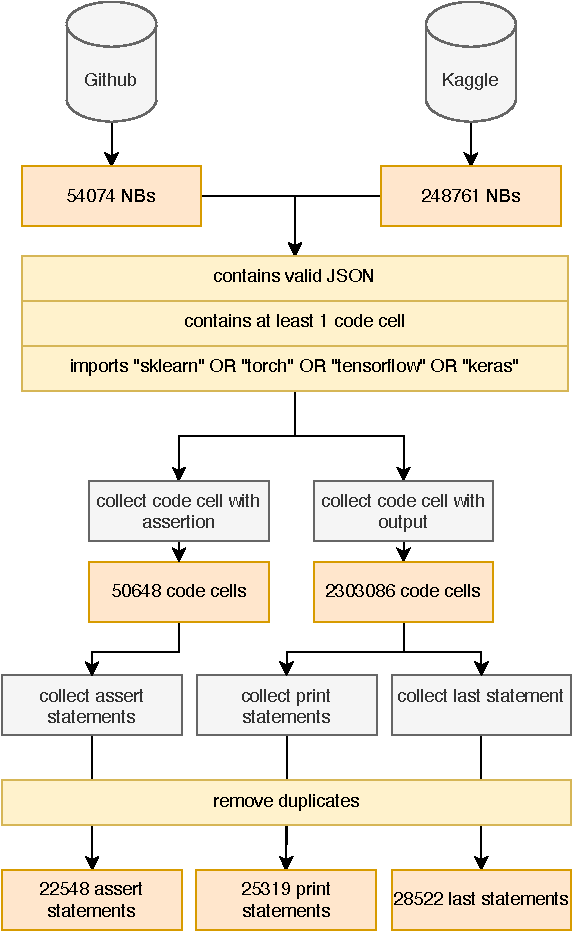
\includegraphics[width=\linewidth]{data-collection.pdf}
\label{fig:data-collection}
\caption{Overview of data collection methodology used in this study}
\end{figure}

Figure~\ref{fig:data-collection} summarises the data collection procedure used in this study. We collected Jupyter notebooks written in Python, from Kaggle and Github. 

We mined public repositories from Github to collect $49923$ Jupyter notebooks. We use the Github advanced search syntax~\footnote{https://docs.github.com/en/search-github/searching-on-github/searching-code} to isolate Jupyter Notebook that contain the keyword ``assert'' in them. The final search query is as follows: \texttt{"assert" language:"Jupyter Notebook"}.\footnote{Collected on June 22, 2023}

For Kaggle, we used a pre-existing dataset KGTorrent~\cite{quaranta2021kgtorrent} since Kaggle does not support advanced code-based search like Github. To the best of our knowledge, KGTorrent this is the largest dataset of Python Jupyter notebooks obtained from Kaggle consisting of $248763$ notebooks.

Therefore, we start with 283GB of data comprising of $298686$ Python Jupyter notebooks.

We check the validity of the underlying JSON structure in each notebook using the nbformat tool ~\footnote{https://nbformat.readthedocs.io/en/latest/}. Since the focus of this study is on the analysis of Python code, we only include notebooks that contain at least one code cell. Finally, to focus on Python code written specifically for ML projects, we only include notebooks that import popular ML libraries~\footnote{These libraries are derived from white literature---https://www.coursera.org/articles/python-machine-learning-library, https://www.geeksforgeeks.org/best-python-libraries-for-machine-learning, https://www.datacamp.com/blog/top-python-libraries-for-data-science, https://www.kdnuggets.com/2020/11/top-python-libraries-data-science-data-visualization-machine-learning.html, https://lp.jetbrains.com/python-developers-survey-2022}.

For explicit feedback using assertions, we programmatically analyse the JSON structure of the notebooks to isolate code cells. We collect Python assert statements from the code cells by constructing and subsequently parsing the Abstract Syntax Tree (AST) of the source code present in each cell.

Similarly, for implicit feedback, we first isolate code cells that produce an output. The output of a cell may either be from a ``print'' statement or the last statement of the cell. We collect both of them using the AST of the cell.

Finally, we remove duplicate data points (asserts, prints and last statements) resulting in a final data set of $22548$ assertions, $25319$ print statements and $28522$ last statements.

\subsection{Case Studies}

% TODO: might need a visual aid here

We allocated a fixed time resource of 100 hours to conduct the case study analysis of all candidates (assertions and cell outputs). To surface interesting candidates for the case studies, we apply NLP techniques as described below.

% TODO: point out the poor quality of notebooks out there (we have citations for this); and the resulting noise in the assertions/outputs. Thats why we need to apply these techniques to surface unique and interesting candidates!

The assertions and cell outputs are first tokenised---special characters and alpha-numeric words shorter than two characters are removed. Two stop words namely ``assert'' and ``print'' are removed since they appear in all assertions and print statements respectively. The term frequency (TF) for all tokens is calculated and then normalised using their inter-document frequency (IDF) such that tokens that appear less frequently are assigned a higher value.

We apply stratified random sampling to identify the candidates for the case study analysis. The sub-groups are created by adding TF-IDF of the tokens in each candidate to produce an aggregate value. The candidates are then divided into quartiles based on the aggregate value. A candidate is randomly drawn from each bin and analysed as an in-depth case study. The analysis is stopped when the time resource is exhausted.

During each case study, we analyse the code of the candidate to understand its purpose. Additionally, we analyse the entire code cell, the previous cell, next cell and the notebook's purpose to bring in rich context.

\section{Results}

% TODO: some sort of introduction to the following sub-sections here; we need to explain that for code cell outputs we try to show the python statement that produces the output along with the actual output. Somethimes actual output is not possible (eg. P68) because the statement may be inside an if statement.

\subsection{(RQ1) How is feedback from the output of code cells used when writing ML code in Jupyter notebooks?}~\label{sec:result-rq1}

\subsubsection{Data distribution check ($N = 7$)}~\label{sec:data-distribution-output}
% (O2, O4, O9, O14, O20, O25, O48)

\begin{table}
  \centering
  \caption{Examples of cell outputs used to verify distribution of data.}
  \begin{tabular}{@{}m{0.05\textwidth} m{0.4\textwidth} m{0.4\textwidth}@{}}
    \toprule
    \emph{\textbf{Key}}&
    \emph{\textbf{Code}}&
    \emph{\textbf{Visual Output}}\\
    \midrule

    O2&
    \lstinline[]$_ = sns.catplot(x='category_id', y='likes', data=train, height=5, aspect=1.5)$&
    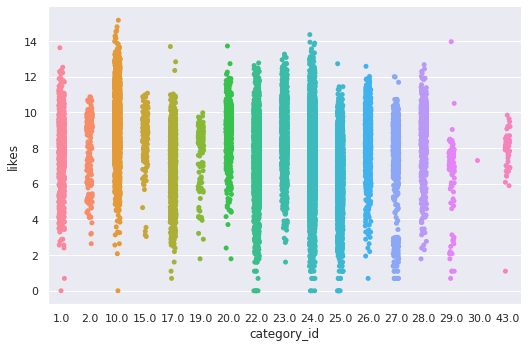
\includegraphics[width=\linewidth]{distribution-check-catplot.png}\\

    O9&
    \lstinline[]$sns.kdeplot(data=data.loc[ data['Survived'] == 0].Age, label='Died', shade=True)$&
    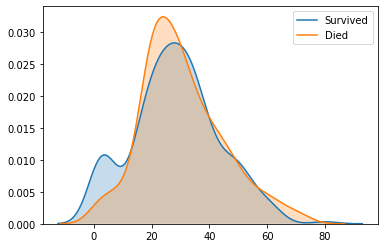
\includegraphics[width=\linewidth]{distribution-check-kdeplot.png}\\

    O14&
    \lstinline[]$pd.pivot_table(train, index='Survived', values=['Age', 'SibSp', 'Parch', 'Fare'])$&
    \\

    O25&
    \lstinline[]$sns.countplot(house_pred['OverallQual'])$&
    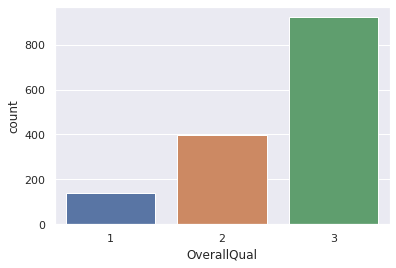
\includegraphics[width=\linewidth]{o25.png}\\

    O48&
    \lstinline[]$x_train.describe()$&
    \\

    \bottomrule
  \end{tabular}
  \label{tab:distribution-check}
\end{table}

Table~\ref{tab:distribution-check} shows examples of outputs used to check the distribution of the data. In output \emph{O2} the distribution of feature \texttt{Age} is checked against the two labels (\texttt{Survived} and \texttt{Died}) of the target feature. Output \emph{O9} presents another example where the distribution of a continuous feature \texttt{likes} is checked with-respect-to all the values of another categorical feature \texttt{category\_id}. Output \emph{O14} produces a pandas dataframe which is used to check the mean value of the features \texttt{Age}, \texttt{SibSp}, \texttt{Parch} and \texttt{Fare} against each label in the target feature \texttt{Survived}. Output \emph{O48} produces a pandas dataframe with the descriptive statistics of all features in the training data. The statement is written immediately after normalising the features in the training data. Hence, the user manually verifies if the normalisation was successful by looking at the mean and standard deviation of the features in the output. Similarly, \emph{O25} is written after discretizing a continuous feature \texttt{OverallQual} using binning. 

Understanding the distribution of data is crucial for making informed decisions about necessary transformation steps in data analysis. For instance, visualizations can efficiently determine if scaling, normalizing, or handling outliers is needed. During the exploratory data analysis (EDA) phase, visualizations and pandas dataframes are commonly used to assess specific columns' distribution, helping identify features related to the target variable and informing feature inclusion in model training. Additionally, descriptive statistics are used post-transformation to verify the effectiveness of steps like data normalization, ensuring data conforms to the expected format for further analysis.

\highlight{\textbf{Finding 1.1} The study identifies seven outputs used to check data distribution, including visualizations like categorical plots, KDE plots, and count plots (O2, O9 and O25), and statistical summaries from pandas dataframes (O14 and O48). These checks are used for making informed decisions about data transformations such as scaling, normalizing and handling outliers, ensuring data integrity and improving model training reliability during the EDA phase.}

\subsubsection{Data relationship check ($N = 2$)}~\label{sec:linear-relation-output}
% (O6, O10)

\begin{table}
  \centering
  \caption{Cell outputs used to verify linear relationship between features in the data.}
  \begin{tabular}{@{}m{0.05\textwidth} m{0.4\textwidth} m{0.4\textwidth}@{}}
    \toprule
    \emph{\textbf{Key}}&
    \emph{\textbf{Code}}&
    \emph{\textbf{Output}}\\
    \midrule

    O6&
    \lstinline[]$b = sns.relplot(x='SIZE', y='Cash', hue='CLARITY', alpha=0.9, palette='muted', height=8, data=raw_data)$&
    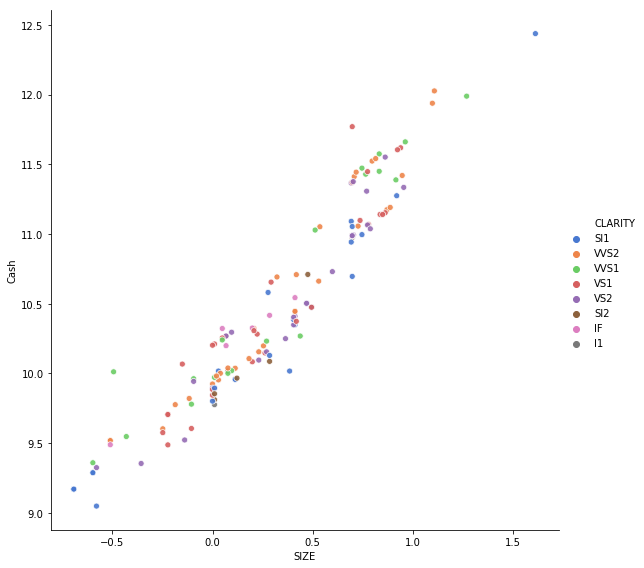
\includegraphics[width=\linewidth]{linear-relation-check-lineplot.png}\\

    O10&
    \lstinline[]$sns.regplot(x='X4 number of convenience stores', y='Y house price of unit area', data=data)$&
    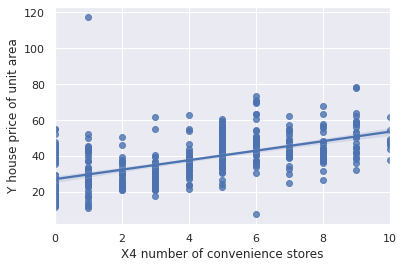
\includegraphics[width=\linewidth]{linear-relation-check-regplot.png}\\
    \bottomrule
  \end{tabular}
\label{tab:linear-relation-check}
\end{table}

Table~\ref{tab:linear-relation-check} illustrates two outputs found in this study for identifying linear relationships amongst features in the data. In output \emph{O6}, the practitioner assesses the linearity between the features \texttt{Cash} and \texttt{SIZE}. Output \emph{O10} depicts the visualization of the feature \texttt{X4} alongside the target variable \texttt{Y}, accompanied by a fitted linear regression model.

Linear machine learning models achieve optimal performance when the target variable can be expressed as a linear combination of the input features. However, features within a dataset that exhibit a linear relationship are considered redundant as they convey the same information to the model during training. Consequently, the feature engineering stage often involves removing such features to create a more efficient training dataset~\ref{shome2022data}.

\highlight{\textbf{Finding 1.2} The study identifies two outputs used to verify linear relationships between features in the data. Visualizations such as a scatter plot with a regression line (O10) and a line plot (O6) are employed to assess the linearity between features. These checks are used for identifying and potentially removing redundant features or performing feature selection to ensure that the training dataset is optimized for linear ML models.}

\subsubsection{Resource check ($N = 7$)}\label{sec:implicit-resource-check}
% (P71, P86, O64, O66, P68, P82, P107)

\begin{table}
  \centering
  \caption{Examples of cell outputs used to verify if different types of resources are available on the system where the notebook is being executed.}
  \begin{tabular}{@{}m{0.05\textwidth} m{0.8\textwidth}@{}}
    \toprule
    \emph{\textbf{Key}}&
    \emph{\textbf{Code}}\\
    \midrule

    P68&
    \lstinline[]$print('GPU is available')$\\

    P71&
    \lstinline[]$print('Hub version: ', hub.__version__)$\\

    P82&
    \lstinline[]$print('Running on TPU ', tpu.master())$\\

    P86&
    \lstinline[]$print('Cuda is available')$\\

    P107&
    \lstinline[]$print('Model loaded')$\\

    O64&
    \lstinline[]$full_table.head(-5)$\\

    O66&
    \lstinline[]$prostate_cancer_df.shape$\\
    \bottomrule
  \end{tabular}
  \label{tab:resource-check}
\end{table}

% NOTE: O107 is a print statement which is execute even if the prior statement that loads the model fails...
Table~\ref{tab:resource-check} presents outputs used to verify availability of resources on the system in which the notebook is being executed. Outputs \emph{P68}, \emph{P82} and \emph{P86} check for the availability of compute resources, such as a GPU or a TPU. This study also finds outputs used to verify that a dataset or a pre-trained model has been successfully loaded into memory. For example, Output \emph{P107} is written after loading a pre-trained model is loaded into memory. Output \emph{O64} generates a pandas dataframe with the last five rows of the data while \emph{O66} shows the shape of the data. These statements are written directly after loading the data from the file system to manually verify that the data was loaded without errors.

Additionally, print statement \emph{P71} is used to ensure that a certain version of an external library is present on the system. This is interesting since external dependencies in Python projects are typically managed using dependency management solutions such as a \emph{requirements.txt}~\footnote{https://pip.pypa.io/en/stable/reference/requirements-file-format/} file or external tools such as \emph{pipenv}~\footnote{https://pipenv.pypa.io/en/latest/} and \emph{poetry}~\footnote{https://python-poetry.org/}.

\highlight{\textbf{Finding 1.3} The study identifies seven outputs used to verify resource availability on the systems where the Jupyter notebooks are being executed. These checks include confirming the availability of compute resources like GPUs and TPUs (P68, P82 and P86), ensuring datasets or pre-trained models are successfully loaded (P107, O64 and O66), and verifying the presence of specific library versions (P71). These checks are used for ensuring that the computational environment is correctly set up, preventing execution errors, and facilitating smooth workflow execution.}

\subsubsection{Execution time check ($N = 1$)}
% (P66)

\begin{table}
  \centering
  \caption{Print statement used to check the total execution time of training and cross-validating an ML model.}
  \begin{tabular}{@{}m{0.05\textwidth} m{0.8\textwidth}@{}}
    \toprule
    \emph{\textbf{Key}}&
    \emph{\textbf{Code}}\\
    \midrule

    P66&
    \lstinline[]$print('Total Run Time:')$\\
    \bottomrule
  \end{tabular}
  \label{tab:exec-time}
\end{table}

Table~\ref{tab:exec-time} presents print statement \emph{P66} that prints the total execution time of a code cell which trains an ML model with various hyper-parameter configurations using a grid-search. \emph{P66} is also used in other code cells in the notebook that train other ML models.

While training multiple machine learning models for a single task is common, choosing the best model considers not only its performance but also its training speed. Faster training times are more cost-effective for iterative tasks and promote sustainability in the long run~\cite{CITEME}.

\highlight{\textbf{Finding 1.4} The study identifies one output (P66) used to check the total execution time of training and cross-validating an ML model. The print statement is used for evaluating the efficiency of model training processes, especially when multiple models are trained iteratively.} 

\subsubsection{Missing value check ($N = 3$)}
% (O12, O36, P74)

\begin{table}
  \centering
  \caption{Examples of cell outputs used to check for missing data.}
  \begin{tabular}{@{}m{0.05\textwidth} m{0.4\textwidth} m{0.4\textwidth}@{}}
    \toprule
    \emph{\textbf{Key}}&
    \emph{\textbf{Code}}&
    \emph{\textbf{Visual Output}}\\
    \midrule

    P74&
    \lstinline[]$print(train_df.isnull().sum())$\\

    O12&
    \lstinline[]$sns.heatmap(test_df.isnull(), yticklabels=False, cbar=False, cmap='viridis')$&
    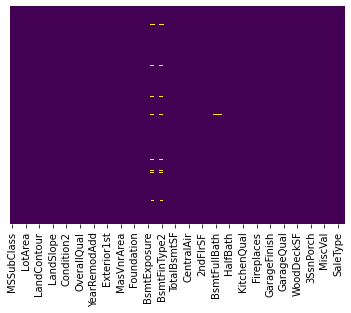
\includegraphics[width=\linewidth]{missing-value-check.png}\\

    O36&
    \lstinline[]$test.isna().sum().unique()$\\
    \bottomrule
  \end{tabular}
  \label{tab:missing-value}
\end{table}

Table~\ref{tab:missing-value} presents all case studies where cell outputs were used to check for missing data. While \emph{P74} and \emph{O36} perform this check in code, \emph{O12} presents a visual representation of missing data using a heatmap.

Checking for missing values is a critical step in the preprocessing phase of a machine learning project because it significantly influences the quality and performance of the model. Missing data can lead to biased or incorrect conclusions if not handled properly, potentially skewing the model's performance by training on incomplete or non-representative samples~\cite{shome2022data}. Many machine learning algorithms, including those that involve matrix multiplication operations such as linear regression and neural networks, demand complete numerical datasets to perform calculations. Missing values interrupt these calculations, leading to errors or the inability to execute algorithms entirely.

\highlight{\textbf{Finding 1.5} The study identifies three outputs (P74, O12 and O36) used to check for missing data. Missing values can lead to biased or incorrect conclusions, and many ML algorithms require complete numerical datasets for accurate calculations. Identifying and addressing missing data during preprocessing is essential to avoid errors and improve model reliability.}

\subsubsection{Model performance check ($N = 33$)}
% (O3, O50, O52, O57, O74, P3, P6, P8--12, P16--19, P23, P24, P28, P30, P34, P42, P47, P48, P50, P51, P54, P55, P57, P58, P61, P78, P93)

\begin{table}
  \centering
  \caption{Various cell outputs used to check the performance of an ML model after training.}
  \begin{tabular}{@{}m{0.05\textwidth} m{0.4\textwidth} m{0.4\textwidth}@{}}
    \toprule
    \emph{\textbf{Key}}&
    \emph{\textbf{Code}}&
    \emph{\textbf{Visual Output}}\\
    \midrule

    P3&
    \lstinline[]$print('The mean accuracy with 10 fold cross validation is: %s ' % round(scores * 100, 2), '%')$&
    \\

    P6&
    \lstinline[]$print('RMSE:', np.sqrt(metrics.mean_squared_error(y_test, pred)))$&
    \\

    P18&
    \lstinline[]$print('The Accuracy is:', accuracy_score(y_test, y_pred))$&
    \\

    P50&
    \lstinline[]$print('Classification Report: SVM (validation data)')$&
    \\

    P54&
    \lstinline[]$print('Intercept value:', lm.intercept_)$&
    \\

    O3&
    \lstinline[]$skplt.metrics. plot_confusion_matrix(Y_val, Vote.predict(X_val), normalize=True, figsize=(10, 10))$&
    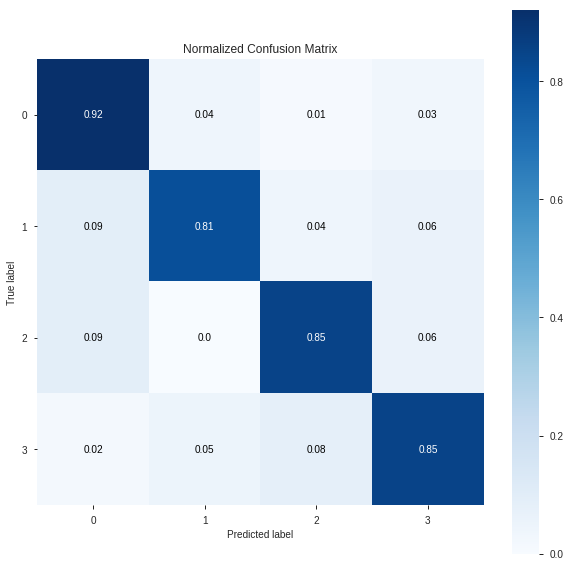
\includegraphics[width=\linewidth]{model-perf-confusion-matrix.png}\\

    O52&
    \lstinline[]$spot_check_recs(classifier, 910)$&
    \\
    \bottomrule
  \end{tabular}
  \label{tab:model-perf}
\end{table}

Table~\ref{tab:model-perf} presents a few examples of cell outputs used to check the performance of a trained ML model. Besides the \emph{accuracy} of the model (\emph{P3} and \emph{P18}), we also see checks for the \emph{Root Mean Square Error (RMSE)} (\emph{P6}) and the use of the classification report (\emph{P50}) provided by scikit-learn~\footnote{https://scikit-learn.org/stable/modules/generated/sklearn.metrics.classification\_report.html} which reports the \emph{accuracy}, \emph{precision}, \emph{recall} and \emph{f1 score} for all labels present in the target feature.

% TODO: this feels hallucinated; revisit
Print statement \emph{P54} prints the intercepts of a linear regression model. Checking the intercept of a linear regression model is essential for understanding the baseline prediction when all predictors are zero, interpreting the model, identifying potential data biases or missing variables, assessing model validity, and comparing baseline predictions across different models. This insight is critical for accurate model interpretation and effective decision-making in practical applications.

Output \emph{O3} shows a heatmap used to visualise the confusion matrix of a multi-label classification task. The values are normalised using the actual number of examples of each class which makes the comparisons of the values across the classes possible.

Output \emph{O52} shows a function implemented by the practitioners to manually evaluate an image classification model on a random sample of input images. The function \texttt{spot\_check\_recs} displays the input image along with the prediction of the model which the practitioner uses to spot-check the performance of the model.

During the model development phase, the performance of an ML model is often printed to facilitate comparisons against other models or variations. Throughout this continuous experimentation phase, authors may adjust model parameters or modify the data by engineering new features. The model is then re-trained to check if these changes lead to performance improvements.

\highlight{\textbf{Finding 1.6} The study identifies 33 outputs used to check the performance of trained ML models. These include outputs that print key performance metrics (P3, P6, P18, P50), a normalised heatmap used to visualise the confusion matrix of a model's predictions (O3) and a custom function written for manual evaluation of model predictions on random input samples (O52). These checks are used throughout the iterative model development phase, enabling practitioners to compare different models or variations, adjust parameters, and refine features to improve performance.}

\subsubsection{Neural network architecture ($N = 1$)}
% (P92)

\begin{table}
  \centering
  \caption{Print the architecture of a neural network.}
  \begin{tabular}{@{}m{0.05\textwidth} m{0.8\textwidth}@{}}
    \toprule
    \emph{\textbf{Key}}&
    \emph{\textbf{Code}}\\
    \midrule
    P92&
    \lstinline[]$print(MyNetwork)$\\
    \bottomrule
  \end{tabular}
  \label{tab:network-architecture}
\end{table}

% TODO: need more description and context around this print statement (where was it written, and why?)
Table~\ref{tab:network-architecture} shows print statement \emph{P92} which shows the architecture of a neural network.

Printing the structure of a neural network serves crucial purposes such as verifying the correct implementation of the architecture, aiding in debugging by ensuring layer compatibility, and providing a clear, human-readable format for documentation and educational insights. It helps in verifying configurations like layer dimensions and operations before initiating computationally intensive training, ensuring the model is set up efficiently for the intended tasks. This practice is fundamental for maintaining accuracy, facilitating collaboration, and enhancing the reproducibility of the model.

\highlight{\textbf{Finding 1.7} The study identifies one output (P92) used to print the architecture of a neural network. Such outputs can be used during the model development phase to ensure compatibility between the layers of a neural network, for understanding and learning about the architecture of pre-trained models and for documentation purposes.}

\subsubsection{Shape check ($N = 3$)}
% (P4, P32, P117)

\begin{table}
  \centering
  \caption{Example of outputs used to check the shape of the data.}
  \begin{tabular}{@{}m{0.05\textwidth} m{0.8\textwidth}@{}}
    \toprule
    \emph{\textbf{Key}} & \emph{\textbf{Code}}\\
    \midrule
    P4 &
    \lstinline[]$print('no.of examples in test data : ', len(test_data))$\\

    P32 &
    \lstinline[]$print('Training set shape : ', x_train.shape)$\\

    P117&
    \lstinline[]$print('Y_train.shape: ', Y_train.shape)$\\
    \bottomrule
  \end{tabular}
  \label{tab:shape-check}
\end{table}

Table~\ref{tab:shape-check} shows print statements discovered in this study which check the shape of the data. \emph{P4} prints the number of rows or examples in the test set. \emph{P32} and \emph{117} prints the number of rows and columns (or features) in the training and test data respectively.

Ensuring that data dimensions align with expectations is important particularly following data pre-processing or transformation steps. Primarily, the number of features in the training set must match those in the testing set. This alignment is crucial because statistical machine learning models are trained on specific data dimensions and expect the same dimensional structure during inference to perform accurately. Similarly, in neural network architectures, the configuration of input layers depends directly on the shape of the training data, dictating the number of input neurons needed. Furthermore, the correspondence between the number of test examples and their respective labels is essential for accurately computing performance metrics, such as accuracy.

Such checks are indicative of the meticulous attention to detail necessary in the model training and validation process, underscoring the importance of shape validation in achieving reliable machine learning outcomes.

\highlight{\textbf{Finding 1.8} The study identifies three outputs used to check the shape of data. These checks are used to ensure data dimensions align with expectations, particularly after preprocessing or transformation steps.}

\subsubsection{Type check ($N = 2$)}
% (O71, P43)

% TODO: the narrative is not as strong here; it would help to also show the actual output as well? For instance, in P43 by itself doesn't make that much sense, the output however shows that all features in the dataset are floats which is a pre-requisite for ML training data
\begin{table}
  \centering
  \caption{Outputs used to check the data type of features in the data.}
  \begin{tabular}{@{}m{0.05\textwidth} m{0.8\textwidth}@{}}
    \toprule
    \emph{\textbf{Key}} &
    \emph{\textbf{Code}}\\

    P43&
    \lstinline[]$print('data type:', images.dtype)$\\

    O71&
    \lstinline[]$type(Y)$\\
    \bottomrule
  \end{tabular}
  \label{tab:type-check}
\end{table}

% TODO: for O71, the output shows its a ndarray; without showing this to the reader we cannot make a strong narrative around these type checks
Table~\ref{tab:type-check} illustrates outputs of cells found in our analysis, where checks are employed to verify the data types of the features in the dataset. Print statement \emph{P43} is written prior to training a neural network. The output validates that all features in the training data are numerical. Similarly, output \emph{O71} shows the data type of the target column.

Type checks are crucial not only for confirming the current state of the data but also for determining the specific transformations required to make the data suitable for subsequent modelling steps. Ensuring data types align with model requirements is a fundamental step in the exploratory data analysis (EDA) phase of developing machine learning models. Since all machine learning algorithms perform mathematical operations, such as matrix multiplications, they require the input data to be entirely numerical to avoid computational errors. The process of checking data types helps in identifying the necessary pre-processing or transformation steps to convert the data into a form that is compatible with these models. For example, while numerical features often require normalisation to bring them within a specific scale, categorical features must be converted into a numerical format through methods like one-hot encoding to ensure they can be effectively integrated into the model.

\highlight{\textbf{Finding 1.9} The study identifies two outputs used to verify the data types of features in the dataset. These checks are used to determine the necessary preprocessing or transformation steps requried to make the data suitable for training. Type checks are also used to ensure that all features are numerical prior to performing mathematical operations such as matrix multiplication, which is used in several ML models.}

\subsubsection{Spot checks ($N = 5$)}
% (O56, O60, P64, P67, P114)

\begin{table}
  \centering
  \caption{Example of outputs used to perform spot checks.}
  \begin{tabular}{@{}m{0.05\textwidth} m{0.8\textwidth}@{}}
    \toprule
    \emph{\textbf{Key}}&
    \emph{\textbf{Code}}\\
    \midrule

    O60 &
    \lstinline[]$X_pca.head()$\\

    P64 &
    \lstinline[]$print(np.max(cur[:, :, 1]))$\\

    P114 &
    \lstinline[]$print(onehot_encoded)$\\
    \bottomrule
  \end{tabular}
  \label{tab:spot-check}
\end{table}

Table~\ref{tab:spot-check} presents outputs which were used to perform spot checks at various stages of the ML development cycle. In \emph{O60}, the practitioner verifies that the number of features in the data matches expectations after apply Principal Component Analysis (PCA). \emph{P64} demonstrates another case which is particularly relevant in image processing contexts. The maximum value in the second channel of a 3D numpy array is extracted and verified, ensuring that the data manipulation retains its expected properties. Lastly, \emph{P114} assesses the correctness of one-hot encoding, a fundamental preprocessing step for categorical data, ensuring that the transformation has been executed correctly.

Performing value or spot checks can be an essential practice for ensuring data integrity and model accuracy at various stages of development. These checks are crucial for verifying that operations such as data transformations, model predictions, and feature engineering are functioning as expected. Each of these checks not only validates individual transformations or predictions but also reinforces the overall reliability and robustness of the machine learning models being developed.

\highlight{\textbf{Finding 1.10} This study finds five outputs used to perform spot checks at various stages of the MLDL. Spot checks are used to ensure data integrity by verifying data transformation and feature engineering steps meet expectations.}

\subsubsection{Model training ($N = 4$)}
% (O8, O31, O42, P77)

\begin{table}
  \centering
  \caption{Example of outputs used to monitor model training.}
  \begin{tabular}{@{}m{0.05\textwidth} m{0.8\textwidth}@{}}
    \toprule
    \emph{\textbf{Key}}&
    \emph{\textbf{Code}}\\
    \midrule

    O8 &
    \lstinline[]$autoencoder.fit(x=X_train, y=X_train, epochs=15, validation_data=[X_test, X_test], callbacks=[keras_utils.TqdmProgressCallback()], verbose=0)$\\

    O31 &
    \lstinline[]$adaBoost.fit(X_train, y_train)$\\

    O42&
    \lstinline[]$m_r.best_params_$\\
    \bottomrule
  \end{tabular}
  \label{tab:model-training}
\end{table}

During training it is common practice to monitor progress periodically, as illustrated by outputs \emph{O8} in Table~\ref{tab:model-training}, where the training loss and accuracy are printed to give real-time feedback on the model's learning efficacy. This feedback allows for adjustments in training parameters or early stopping to prevent overfitting. For instance, in output O8, the autoencoder is trained using a custom callback from \texttt{keras\_utils} to provide a progress update without cluttering the output stream, which is particularly useful in lengthy training sessions. In contrast, output \emph{O31} represents a crucial validation step where the \texttt{adaBoost} model is fitted to the training data to ensure it adheres to the expected data patterns without errors, a typical task in the model experimentation phase where various models are assessed for their suitability. Output \emph{O42} checks for the best parameters found through tuning methods, highlighting the importance of parameter optimisation in achieving optimal model performance.

Each of these outputs underscores different facets of the model training phase, from initialization and real-time monitoring to validation and finalization, illustrating the layered complexity of developing predictive models.

\highlight{\textbf{Finding 1.11} The study identifies four outputs used to monitor model training progress. These outputs provide real-time feedback on training loss and accuracy (O8), validate model adherence to expected data patterns (O31), and identify optimal parameters through tuning methods (O42). These checks facilitate timely adjustments during the training process to prevent overfitting and ensure model performance optimization.}

\subsection{(RQ2) How are assertions used to validate ML code written in Jupyter notebooks?}~\label{sec:result-rq2}

% TODO: bring in the notion of pre and post condition checks (the wikipedia page on assertions is very interesting: https://en.wikipedia.org/wiki/Assertion_(software_development)); specifically the part on run-time assertions

\subsubsection{Batch size check ($N = 3$)}
% (A21, A28, A70)

\begin{table}
  \centering
  \caption{Assertions used to validate the batch size of input data.}
  \begin{tabular}{@{}m{0.05\textwidth} m{0.8\textwidth}@{}}
    \toprule
    \emph{\textbf{Key}}&
    \emph{\textbf{Code}}\\
    \midrule

    A21 &
    \lstinline[]$assert x.size(0) % batch_size == 0, f'the first dimension of input tensor ({x.size(0)}) should be divisible by batch_size ({batch_size})'$\\

    A28 &
    \lstinline[]$assert image_size % patch_size_small == 0, 'Image dimensions must be divisible by the patch size.'$\\

    A70 &
    \lstinline[]$assert n_img > batch_size$\\
    \bottomrule
  \end{tabular}
  \label{tab:batch-size}
\end{table}

Table~\ref{tab:batch-size} shows the assertions found in this study that validate the batch size. \emph{A21} ensure that the batch size divides evenly into the training dataset size, thereby confirming that every training epoch processes full batches without leftover data. Similarly, \emph{A28} checks that image dimensions are suitably divisible by the patch size, which is essential for certain types of convolutional networks. \emph{A70} is another critical check which confirms that the number of images is greater than the batch size, which is necessary to commence batch processing.

In the context of neural network training, the practice of using batch processing is a key strategy to enhance computational efficiency and hardware utilization, particularly GPU cores. Batching allows for a more stable and smoother learning curve as the model's weights are updated not for each individual example, but rather based on the average gradient of a batch. This technique not only optimizes learning but also enhances the model's generalizability due to more robust gradient estimations. Given these benefits, it becomes crucial to ensure that the batch size is appropriately set to match the hardware's capacity, avoiding memory overflow issues that can halt training. These assertions are strategically placed to prevent common errors that could undermine training efficiency and model performance, thereby safeguarding the training process from potential disruptions due to misconfigured batch sizes.

\highlight{\textbf{Finding 2.1} This study identifies three assertions validating batch size configurations. These assertions ensure batch sizes are divisible by dataset sizes, image dimensions are appropriately divided by patch sizes, and the number of images exceeds the batch size. These checks are crucial for optimizing computational efficiency and ensuring stable and smooth model training.}

\subsubsection{Data leakage check ($N = 1$)}
% (A33)

\begin{table}
  \centering
  \caption{Assert used to prevent data leakage.}
  \begin{tabular}{@{}m{0.05\textwidth} m{0.8\textwidth}@{}}
    \toprule
    \emph{\textbf{Key}}&
    \emph{\textbf{Code}}\\
    \midrule

    A33&
    \lstinline[]$assert len(set( tr_df.PetID.unique()).intersection(valid_df.PetID.unique())) == 0$\\
    \bottomrule
  \end{tabular}
  \label{tab:data-leakage}
\end{table}

Assertion \emph{A33} in Table~\ref{tab:data-leakage} ensures that there are no overlapping \texttt{PetID} values between the training set \texttt{tr\_df} and the validation set \texttt{valid\_df}, thereby preventing any possibility of data leakage.

Ensuring the absence of data leakage between training and validation datasets is a fundamental best practice in machine learning to prevent models from overfitting. Overfitting occurs when a model is excessively complex, learning not only the underlying patterns but also the noise in the training data, which can degrade its performance on unseen data. To guarantee that the model can generalize effectively to new examples, it's crucial to verify that the training and validation sets are completely distinct with no shared examples. By strictly separating these datasets, the validation phase serves its purpose of providing an unbiased evaluation of the model's ability to generalize---to data similar to, but not identical to that which it was trained on---thus maintaining the integrity and validity of the evaluation metrics derived during model testing.

\highlight{\textbf{Finding 2.2} This study identifies one assertion to ensure there are no overlapping values between training and validation sets to prevent data leakage. Preventing data leakage is essential to avoid overfitting and ensure the model's ability to generalize to new data. This practice maintains the integrity and validity of the model evaluation metrics.}

\subsubsection{Existence check ($N = 8$)}
% NOTE: this is a combination of missing-value-check and existence-check
% (A23, A42, A43, A50, A51, A63, A79, A86)

\begin{table}
  \centering
  \caption{Assertions used to perform existence checks.}
  \begin{tabular}{@{}m{0.05\textwidth} m{0.8\textwidth}@{}}
    \toprule
    \emph{\textbf{Key}}&
    \emph{\textbf{Code}}\\
    \midrule

    A23 &
    \lstinline[]$assert np.all(orders.groupby('user_id') .days_since_prior_order.tail(1).notnull())$\\

    A42 &
    \lstinline[]$assert not lab_s.isnull().values.any()$\\

    A43 &
    \lstinline[]$assert len(data) != 0, 'cannot divide by zero'$\\

    A50 &
    \lstinline[]$assert not np.any(np.isnan(X))$\\

    A51 &
    \lstinline[]$assert data.target.notnull().all()$\\

    A63 &
    \lstinline[]$assert X.isnull().sum().sum() == 0$\\

    A79 &
    \lstinline[]$assert not processed_data_df.isna().any().any()$\\

    A86 &
    \lstinline[]$assert p0 in poi_info.index$\\
    \bottomrule
  \end{tabular}
  \label{tab:existence-check}
\end{table}

Assertions \emph{A23} and \emph{A42} in Table~\ref{tab:existence-check} ensure that specific data columns do not contain any missing entries, which could compromise the reliability of subsequent analyses. Assertion \emph{A43} guards against operations on empty datasets, which are a potential risk after filtering or merging data processes. Assertions \emph{A50}, \emph{A51} and \emph{A63} rigorously confirm that the datasets are entirely free from \texttt{NaN} values, thus preserving the integrity of the dataset for reliable model training. Assertions \emph{A79} and \emph{A86} ensure that no unexpected missing values are introduced and that all expected indices are present in the dataset respectively.

Existence checks are a fundamental component of data preprocessing in ML, serving multiple critical purposes to ensure data integrity before analysis and modeling. These checks primarily focus on verifying the presence of necessary columns and the absence of missing values within those columns. Such validations are especially crucial after data preprocessing steps, where transformations might inadvertently introduce null values. These checks are also crucial for maintaining the accuracy and efficiency of data handling processes, ensuring that the datasets are ready for robust machine learning applications.

\highlight{\textbf{Finding 2.3} Eight assertions ensure the presence of specific columns in the dataset and the absence of missing values. These checks prevent operations on empty datasets and confirm the absence of \texttt{NaN} values, maintaining data integrity and reliability for model training.}

\subsubsection{Mathematical property checks ($N = 4$)}
% (A3, A25, A56, A64)

\begin{table}
  \centering
  \caption{Assertions used to validate mathematical properties of neural networks.}
  \begin{tabular}{@{}m{0.05\textwidth} m{0.8\textwidth}@{}}
    \toprule
    \emph{\textbf{Key}}&
    \emph{\textbf{Code}}\\
    \midrule

    A3 &
    \lstinline[]$assert (xH - wH) % self.stride == 0$\\

    A25 &
    \lstinline[]$assert test_output.std() < 0.15, "Don't use batchnorm here"$\\

    A56 &
    \lstinline[]$assert np.allclose(e_v_states[:, -1], np.ones_like(e_v_states[:, -1]))$\\

    A64 &
    \lstinline[]$assert np.allclose(T, T.T)$\\
    \bottomrule
  \end{tabular}
  \label{tab:maths-check}
\end{table}

Assertion \emph{A3} in Table~\ref{tab:maths-check} checks that the dimension differences between height of input and the filter, when divided by the stride, result in an integer, ensuring that convolution operations are dimensionally consistent. \emph{A25} monitors the standard deviation of outputs to decide the appropriateness of using batch normalisation, thus guiding the model optimization process based on statistical behavior. \emph{A56} verifies the uniformity of certain computations, essential for maintaining consistency in state or parameter arrays over iterations. Similarly \emph{A64} checks for the symmetry of a matrix, a crucial property in many algorithms, particularly those involving covariance matrices and distance calculations. 

When working with neural networks and other statistical models, it is imperative to ensure that mathematical properties are preserved throughout operations involving arrays and matrices. This rigor is captured through the assertions in Table~\ref{tab:maths-check} tha validate these properties after matrix manipulations. These assertions are not just precautionary but are vital for confirming that the underpinnings of ML algorithms align with expected mathematical principles, thereby ensuring the robustness and reliability of model computations and outcomes.

\highlight{\textbf{Finding 2.4} Four assertions validate key mathematical properties of data and model outputs. These include ensuring dimensional consistency in convolution operations, monitoring standard deviation for batch normalization suitability, verifying uniformity in computations, and checking matrix symmetry. These checks confirm the robustness and reliability of model computations.}

\subsubsection{Model performance check ($N = 11$)}\label{sec:assert-model-perf}
% (A7, A15, A19, A22, A24, A26, A38, A54, A58, A59, A72)

\begin{table}
  \centering
  \caption{Assertions used to check performance of ML models.}
  \begin{tabular}{@{}m{0.05\textwidth} m{0.8\textwidth}@{}}
    \toprule
    \emph{\textbf{Key}}&
    \emph{\textbf{Code}}\\
    \midrule

    A7 &
    \lstinline[]$assert len(neighbours_1) == 20, "Neighbors don't match!"$\\

    A15 &
    \lstinline[]$assert np.allclose(verify('images/camera_1.jpg', 'bertrand', database, FRmodel), (0.54364836, True))$\\

    A19 &
    \lstinline[]$assert np.allclose(linear_model.coef_, [[1.57104472, 0.92521608]]), 'The model parameters you learned seem incorrect!'$\\

    A38 &
    \lstinline[]$assert 0.75 < auc(fpr, tpr) < 0.85$\\

    A58 &
    \lstinline[]$assert np.isclose(accuracy, 0.9666666666666667)$\\
    \bottomrule
  \end{tabular}
  \label{tab:model-perf-explicit}
\end{table}

This study finds several assertions used to test model performance against predefined thresholds for key metrics such as accuracy, precision, recall, F1 score, and others.

% TODO: verify if this applies to recommender systems as well?
For example, \emph{A7} in Table~\ref{tab:model-perf-explicit} checks for the expected number of neighbors as an indirect measure of model performance in specific scenarios like recommendation systems or clustering. Meanwhile, direct comparisons of model outputs with expected results, as seen in \emph{A15} validate the model's predictive accuracy and reliability under operational conditions. Other assertions, such as \emph{A19}, ensure that the learned parameters align closely with theoretically or empirically derived values, further cementing the model’s statistical validity. Range checks like \emph{A38} confirm that the performance metrics such as \emph{AUC} and \emph{Gini coefficient} fall within acceptable boundaries, indicating good predictive performance without overfitting.

The use of \texttt{np.isclose} in \emph{A58} is particularly noteworthy. This method accounts for the stochastic nature of many ML models, where slight variations in performance metrics can occur due to differences in initial conditions, random seed settings, or inherent randomness in algorithms. By allowing a small tolerance in the comparison, np.isclose ensures that the model's performance is consistently close to the expected benchmark, thereby affirming its reliability despite the stochastic elements.

\highlight{\textbf{Finding 2.5} Eleven assertions evaluate model performance against predefined thresholds for accuracy, precision, recall, F1 score, and other metrics. These checks validate the model's predictive accuracy and reliability, ensuring it meets expected performance standards despite the stochastic nature of ML models.}

\subsubsection{Network architecture check ($N = 3$)}
% (A11, A62, A75)

\begin{table}
  \centering
  \caption{Assertions used to check the architecture of neural networks.}
  \begin{tabular}{@{}m{0.05\textwidth} m{0.8\textwidth}@{}}
    \toprule
    \emph{\textbf{Key}}&
    \emph{\textbf{Code}}\\
    \midrule

    A11 &
    \lstinline[]$assert self.encoder_conv_01[0].weight.size() == self.vgg16.features[2].weight.size()$\\

    A62 &
    \lstinline[]$assert activations[i + 1].shape[1] == self.encoder_layer_sizes[-1] * 2$\\
    
    A75 &
    \lstinline[]$assert reg in ['none', 'l2']$\\
    \bottomrule
  \end{tabular}
  \label{tab:assert-network-architecture}
\end{table}

Assertion \emph{A11} verifies that the weight dimensions of the first convolutional layer in the \lstinline{encoder_conv_01} module match the weight dimensions of the third layer in the \lstinline{vgg16.features} module. The \lstinline{vgg16} model is a widely-used pre-trained convolutional neural network often employed as a feature extractor or backbone for transfer learning tasks. By ensuring that the weight dimensions are consistent, the code guarantees that the input data to the \lstinline{encoder_conv_01} module has the expected spatial dimensions and number of channels, enabling seamless integration with the pre-trained \lstinline{vgg16} model.

Assertion \emph{A62} checks that the shape of the activations at index \lstinline{i + 1} has the correct number of channels, which should be twice the size of the last encoder layer. This ensures that the intermediate activations maintain the expected structure necessary for the proper functioning of the subsequent layers in the network. Ensuring that the shape of activations is consistent throughout the network is crucial for maintaining the integrity of the data flow and preventing errors during the forward pass.

Assertion \emph{A75} ensures that the regularization parameter \lstinline{reg} is either 'none' or 'l2'. This check is important for validating that the specified regularization method is among the acceptable options, thereby preventing potential misconfigurations that could lead to unexpected behavior or suboptimal model performance.

When integrating pre-trained models or leveraging transfer learning techniques, it is crucial to ensure the compatibility of the custom neural network architecture with the pre-trained components. This is particularly important when combining convolutional layers from different sources, as the spatial dimensions and channel configurations must align correctly. Such architectural checks are crucial for preventing potential issues during the forward pass of the neural network and ensuring that the custom and pre-trained components are compatible, ultimately leading to reliable and accurate model performance.

\highlight{\textbf{Finding 2.6} Three assertions verify the consistency of neural network architecture. These include ensuring weight dimensions match across layers and that activation shapes and regularization parameters are as expected. These checks ensure that the neural network is correctly configured and integrated with pre-trained models, maintaining the integrity of data flow during training.}

\subsubsection{Resource check ($N = 7$)}
% (A10, A14, A18, A37, A60, A67 A74)

\begin{table}
  \centering
  \begin{tabular}{@{}m{0.05\textwidth} m{0.8\textwidth}@{}}
    \toprule
    \emph{\textbf{Key}}&
    \emph{\textbf{Code}}\\
    \midrule

    A10 &
    \lstinline[]$assert le_path.is_file(), f"Label encoder file not found at {le_path}. Make sure 'label_encoder.pkl' exists in the lightning_logs directory."$\\

    A14 &
    \lstinline[]$assert self.model is not None, 'Model is not loaded, load it by calling .load_model()'$\\

    A18&
    \lstinline[]$assert pd.__version__.rpartition('.')[0] == '1.0', f"Unexpected pandas version: expected 1.0, got {pd.__version__.rpartition('.')[0]}"$\\

    A37 &
    \lstinline[]$assert svm.fit_status_ == 0, 'Forgot to train the SVM!'$\\

    A60 &
    \lstinline[]$assert f2.gca().has_data()$\\

    A67&
    \lstinline[]$assert pm.__version__ == '3.9.2'$\\

    A74 &
    \lstinline[]$assert os.path.exists(image_dir)$\\
    \bottomrule
  \end{tabular}
  \caption{Assertions used to validate availability of resources.}
  \label{tab:assert-resource-check}
\end{table}

Table~\ref{tab:assert-resource-check} persents the assertions encountered in this study, that perform resource checks encompassing pre-trained models, data paths, visualizations, and model training status. These checks help prevent runtime errors and ensure the proper execution of code.

One set of assertions verify the existence of files on the file system, such as pre-trained models (\emph{A10}) or data files (\emph{A74}). These checks ensure that the required resources are present before proceeding with subsequent operations, preventing potential issues caused by missing resources.

Additionally, assertions are employed to validate the successful loading of models (\emph{A14}) and the completion of model training processes (\emph{A37}). A unique aspect of working with notebooks is the ability to re-run cells while experimenting, which can lead to unintended consequences. The assertion \emph{A37} addresses this scenario by checking if the SVM model has been properly trained before proceeding with further operations. This check prevents inconsistent model states from executing cells out of order or multiple times.

Assertion \emph{A60} is used to verify the presence of data in visualizations generated using the Matplotlib~\footnote{https://matplotlib.org/} library. These checks are crucial for ensuring that the visualizations accurately represent the underlying data and do not contain empty or incomplete plots, which could lead to misleading interpretations.

Assertions \emph{A18} and \emph{A67} explicitly verify the versions of critical libraries. For instance, \emph{A18} checks that the major version of pandas is precisely what is expected for the notebook’s tasks, ensuring compatibility and preventing errors that could arise from API changes in newer or older versions.

Resource check assertions play a vital role in maintaining the reliability and robustness of the machine learning workflows by ensuring the availability and validity of essential resources, preventing runtime errors, and maintaining the integrity of the data, models, and visualizations.

% NOTE: left over loads, move to implications if required
% In the dynamic and sometimes unstructured environment of Jupyter notebooks, managing dependencies directly within the notebook becomes crucial due to the workflow peculiarities associated with interactive sessions. Unlike traditional software development environments where dependencies are managed through dedicated solutions like dependency management tools or by specifying requirements in a \emph{requirements.txt} file, notebooks often require on-the-fly checks to ensure the correct library versions are loaded to avoid compatibility issues.

% These assertions safeguard the notebook against potential disruptions caused by version mismatches, thereby maintaining the integrity of the codebase and ensuring reproducibility across different execution environments.

\highlight{\textbf{Finding 2.7} Seven assertions confirm the availability of essential resources like pre-trained models, data files, successful model loading, and completion of training processes. These checks prevent runtime errors and ensure proper code execution, maintaining the reliability and robustness of the ML workflows.}

\subsubsection{Data shape check ($N = 26$)}
% (A5, A9, A13, A16, A17, A29, A31, A61, A71, A76--78, A82, A84, A85, A89, A90, A91, A93--96, A98--101)

% TODO: revisit the assertions in this section; we may have misclassified assertions or need to create a new group

\begin{table}
  \centering
  \caption{Assertions used to check the shape of the data.}
  \begin{tabular}{@{}m{0.05\textwidth} m{0.8\textwidth}@{}}
    \toprule
    \emph{\textbf{Key}}&
    \emph{\textbf{Code}}\\
    \midrule

    A5 &
    \lstinline[]$assert y_valid.shape == (1132,)$\\

    A17 &
    \lstinline[]$assert X.shape[1] == 13, 'Did you drop/lose some columns in X? Did you properly load and split the data?'$\\

    A29 &
    \lstinline[]$assert len(test_y_preds) == len(test_y), 'Unexpected number of predictions.'$\\

    A31 &
    \lstinline[]$assert img.shape == (112, 92)$\\

    A76 &
    \lstinline[]$assert len(encoding['token_type_ids']) == max_seq_length$\\

    A84 &
    \lstinline[]$assert red.get_shape().as_list()[1:] == [224, 224, 1]$\\

    A90 &
    \lstinline[]$assert len(X_train) == 2000$\\

    A93 &
    \lstinline[]$assert temp_embed.shape[0] == stride$\\
    \bottomrule
  \end{tabular}
  \label{tab:assert-shape-check}
\end{table}


Assertions \emph{A17} and \emph{A90} verify that the input features have the correct number of columns and examples, respectively. Such checks are essential for preventing downstream errors and ensuring the compatibility of the data with the chosen model architecture and preprocessing steps. 

Assertions \emph{A5} and \emph{A29} ensure that the labels or predictions have the expected length or shape, which is crucial for accurate performance evaluation and model training.

In the context of computer vision tasks, assertions \emph{A31} and \emph{A84} verify that the input images have the correct dimensions, which is essential for compatibility with convolutional neural network architectures and image preprocessing techniques.

Furthermore, assertions \emph{A76} and \emph{A93} check the dimensions of sequences, embeddings, and other data structures used in natural language processing tasks, ensuring their compatibility with various models and algorithms.

Data shape checks can be considered the ``Swiss army knife'' of assertions, as they are ubiquitous and serve multiple purposes throughout the machine learning workflow. We encountered a vast array of assert statements that verify the dimensions of various data structures, including input features, labels, predictions, images, sequences, and embeddings. These assertions ensure that the data adheres to the expected format and dimensions required by different components of the machine learning pipeline.

Data shape check assertions serve as a crucial safeguard against data inconsistencies, ensuring the integrity and compatibility of the data throughout the machine learning workflow. By verifying the expected dimensions and shapes of various data structures, these assertions help prevent runtime errors, ensure accurate model training and evaluation, and maintain the reliability of the entire machine learning pipeline.

\highlight{\textbf{Finding 2.8} 26 assertions verify the dimensions of various data structures such as input features, labels, predictions, images, sequences, and text embeddings. These checks ensure data consistency and compatibility throughout the ML pipeline, preventing runtime errors and ensuring accurate model training and evaluation.}

\subsubsection{Type check ($N = 5$)}
% (A2, A35, A40, A81, A88)

\begin{table}
  \centering
  \caption{Assertions used to check the data type of features in the dataset.}
  \begin{tabular}{@{}m{0.05\textwidth} m{0.8\textwidth}@{}}
    \toprule
    \emph{\textbf{Key}}&
    \emph{\textbf{Code}}\\
    \midrule

    A2 &
    \lstinline[]$assert isinstance(X_trn, torch.FloatTensor), 'Features should be float32!'$\\

    A35 &
    \lstinline[]$assert isinstance(column_transformer, ColumnTransformer), "Input isn't a ColumnTransformer"$\\

    A40 &
    \lstinline[]$assert isinstance(model_3, sklearn.ensemble.RandomForestClassifier)$\\

    A81 &
    \lstinline[]$assert is_all_ints(filled_df[r]) is True$\\

    A88 &
    \lstinline[]$assert isinstance(betas, np.ndarray)$\\
    \bottomrule
  \end{tabular}
  \label{tab:assert-type-check}
\end{table}

Assertion \emph{A2} in Table~\ref{tab:assert-type-check} demonstrates a very common type check performed on the input features. This assertion ensures that the input features are represented as PyTorch float tensors, which is a requirement for many deep learning models and operations.

Another type check is applied to verify the type of the machine learning models themselves. For instance, the \emph{A40} checks if the \lstinline{model_3} object is an instance of the \lstinline{RandomForestClassifier} class from the scikit-learn library. This type of assertion is essential when working with different types of models, as it helps prevent errors arising from using incompatible methods or attributes.

In addition to input features and models, type checks are also performed on data structures and intermediate objects. The assertion \emph{A35} verifies that the \lstinline{column_transformer} object is an instance of the \lstinline{ColumnTransformer} class, which is commonly used for preprocessing and feature engineering tasks in scikit-learn.

Type checking is not limited to objects and data structures--it can also be applied to individual columns or elements within a dataset. The assertion \emph{A81} checks if all the elements in a specific column (\lstinline[]$filled_df[r]$) of a DataFrame are integers.

Furthermore, type checks are performed on NumPy arrays, as demonstrated by the assertion \emph{A88}. This assertion ensures that the \lstinline{betas} object is a NumPy array, which is a fundamental data structure used in many numerical and scientific computing operations.

Type check assertions are essential for maintaining data integrity, ensuring compatibility between different components of the machine learning pipeline, and preventing errors and unexpected behavior. By verifying the types of input features, models, data structures, and other objects, these assertions contribute to the overall reliability and robustness of the machine learning workflow.

\highlight{\textbf{Finding 2.9} Five assertions validate the data types of input features, models, and intermediate objects. These checks ensure compatibility with ML models and operations, preventing errors from incompatible methods or attributes, thus maintaining the reliability of the ML workflow.}

\subsubsection{Data validation check ($N = 14$)}
% formerly value-check (A20, A30, A41, A44--46, A52, A65, A68, A69, A73, A83, A87, A92)

\begin{table}
  \centering
  \caption{Assertions used to perform data validation checks.}
  \begin{tabular}{@{}m{0.05\textwidth} m{0.8\textwidth}@{}}
    \toprule
    \emph{\textbf{Key}}&
    \emph{\textbf{Code}}\\
    \midrule

    A41 &
    \lstinline[]$assert np.all(np.unique(X['smoke'].values) == np.array([0, 1]))$\\

    A44 &
    \lstinline[]$assert abs(min(entity_embedding[low:high]) - max(entity_embedding[low:high])) <= 1$\\

    A46 &
    \lstinline[]$assert np.isclose(stdev_norm, 1.0, atol=1e-16)$\\

    A52 &
    \lstinline[]$assert grouped_users['user_id'].nunique() == user_engagement['user_id'].nunique()$\\

    A65 &
    \lstinline[]$assert np.all(y <= nb_classes)$\\

    A73 &
    \lstinline[]$assert df['clf'].value_counts()[1] == len(df[df['quality'] >= 7])$\\
    \bottomrule
  \end{tabular}
  \label{tab:data-validation}
\end{table}

% TODO: revisit, we have new assertions here; update the count
Table~\ref{tab:data-validation} presents a range of assert statements that perform various validation checks on data structures, such as NumPy arrays and pandas DataFrames. These checks help ensure the data meets specific criteria or constraints, preventing potential errors or inconsistencies in downstream operations.

One type of validation check involves verifying the presence of specific values or ranges within arrays or columns. For example, assertion \emph{A41} checks if the unique values in the \lstinline{smoke} column of the DataFrame \lstinline{X} are limited to 0 and 1. Similarly, \emph{A65} ensures that all values in the array \lstinline{y} are less than or equal to a certain number of classes.

Another common validation check is verifying the equality or closeness of values or arrays. Assertion \emph{A44} checks if the difference between the minimum and maximum values in a specific range of the \lstinline{entity_embedding} array is less than or equal to 1. Assertion \emph{A46} verifies that the \lstinline{stdev_norm} value is close to 1.0 within a specified absolute tolerance.

Some assertions focus on validating the uniqueness or cardinality of values in arrays or DataFrames. For instance, \emph{A52} checks if the number of unique user IDs in the \lstinline{grouped_users} DataFrame is equal to the number of unique user IDs in the \lstinline{user_engagement} DataFrame.

Other assertions validate the presence of specific values or conditions within DataFrames or other data structures. The assertion \emph{A73} checks if the count of a specific value (1) in the ``clf'' column of the DataFrame \lstinline{df} is equal to the number of rows where the ``quality'' column is greater than or equal to 7.

By verifying specific conditions, value ranges, uniqueness, and equality constraints, these assertions help catch potential errors or inconsistencies early in the pipeline, preventing downstream issues and ensuring reliable and accurate results.

\highlight{\textbf{Finding 2.10} Fourteen assertions perform validation checks on data structures, ensuring the presence of specific values, verifying value ranges, and confirming uniqueness or cardinality of values. These checks catch potential errors or inconsistencies early, ensuring data meets specific criteria or constraints for robust ML applications.}

\subsection{(RQ3) How are assertions used to validate visual outputs in Jupyter notebooks?}~\label{sec:result-rq3}

\subsubsection{Model Performance ($N = 15$)}

\begin{longtable}{@{} m{0.05\textwidth} m{0.4\textwidth} m{0.4\textwidth} @{}}
  \caption{VA pairs used to validate the performance of a model.} \\
  \toprule
  \emph{\textbf{Key}} &
  \emph{\textbf{Visual Output}} &
  \emph{\textbf{Assertion}}\\
  \midrule
  \endfirsthead

  \caption[]{VA pairs used to validate the performance of a model (continued).} \\
  \toprule
  \emph{\textbf{Key}} &
  \emph{\textbf{Visual Output}} &
  \emph{\textbf{Assertion}}\\
  \midrule
  \endhead

  \midrule
  \endfoot

  \bottomrule
  \endlastfoot

  VA2 &
  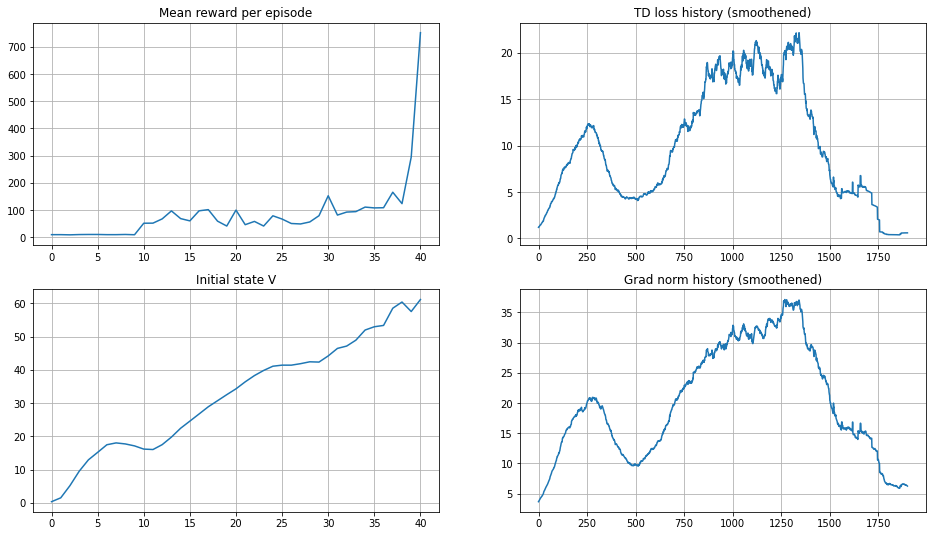
\includegraphics[width=\linewidth]{va2.png} &
  \lstinline[]$assert final_score > 300, 'not good enough for DQN'$\\

  VA3 &
  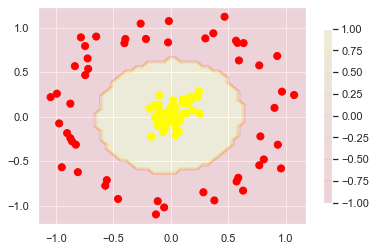
\includegraphics[width=\linewidth]{va3.png} &
  \lstinline[]$assert accuracy_score(y_test, pred) > 0.95$\\

  VA9 &
  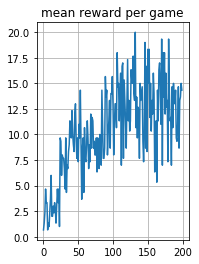
\includegraphics[width=\linewidth]{va9.png} &
  \lstinline[]$assert np.mean(mean_rw_history[-10:]) > 10.$\\

  VA11 &
  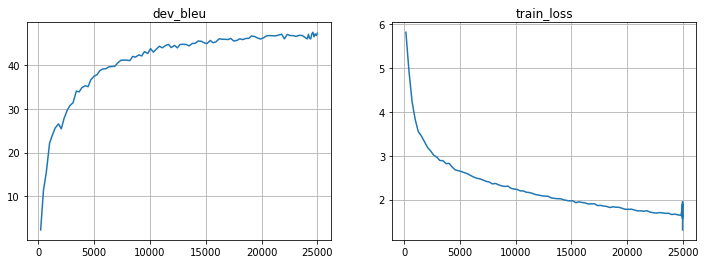
\includegraphics[width=\linewidth]{va11.png} &
  \lstinline[]$assert np.mean(metrics['dev_bleu'][-10:], axis=0)[1] > 35, "We kind of need a higher bleu BLEU from you. Kind of right now."$\\

  VA15 &
  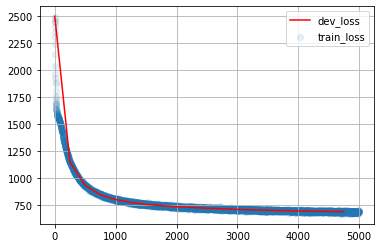
\includegraphics[width=\linewidth]{va15.png} &
  \lstinline[]$assert np.mean(train_history[:10], axis=0)[1] > np.mean(train_history[-10:], axis=0)[1], "The model didn't converge."$\\

  VA28 &
  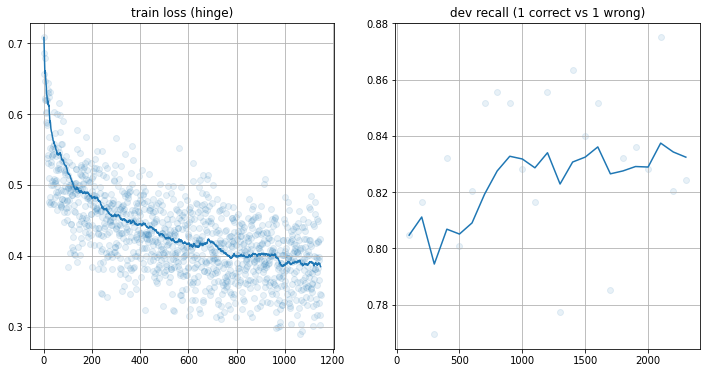
\includegraphics[width=\linewidth]{va28.png} &
  \lstinline[]$assert np.mean(dev_recall_history[-10:]) > 0.85, "Please train for at least 85% recall on test set. You may need to change vectorizer model for that."$\\

  VA68 &
  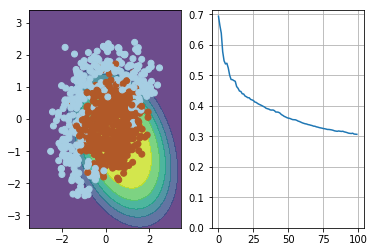
\includegraphics[width=\linewidth]{va68.png} &
  \lstinline[]$np.testing.assert_almost_equal(ans4, 0.3042764)$\\

  VA107 &
  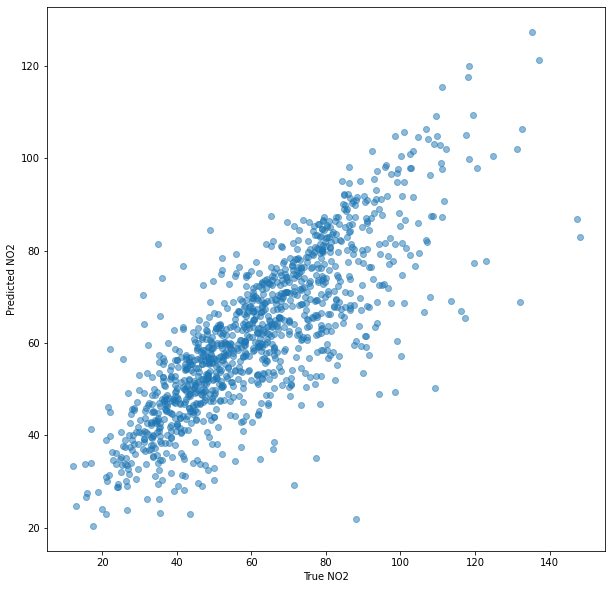
\includegraphics[width=\linewidth]{va107.png} &
  \lstinline[]$assert r2_gru > 0.6$\\

\end{longtable}\label{tab:va-model-perf}

The visualizations in VA2, VA9, and VA15 provide a comprehensive view of key metrics for evaluating the performance of various machine learning models. VA2 includes mean reward per episode, TD loss history, initial state value (V), and gradient norm history for a Deep Q-Network (DQN) model. These metrics collectively indicate the model's learning progress and stability during training. The visualization in VA9 shows the mean reward per game for a DQN applied to the Breakout Atari game, tracking the model's performance over 200 games. The general upward trend indicates learning and improvement in gameplay over time. VA15 presents the training and development loss over time for a character-level language model, showing a gradual decrease in loss and suggesting effective learning.

The visualization in VA3 presents a two-dimensional scatter plot showing the decision boundary of a Support Vector Machine (SVM) model, with red and yellow points representing two different classes and a background color gradient indicating the decision function of the SVM. This visualization aids in understanding the model's ability to distinguish between classes and the distance of the samples from the decision boundary. The visualizations in VA28 display the training loss and development recall, respectively. The left graph shows a decrease in training loss over time, indicating learning progress, while the right graph shows development recall over time, highlighting improvements in the model's ability to correctly identify positive instances. The visualizations in VA11 depict key metrics for evaluating the performance of a machine learning model in text generation or machine translation. The left plot shows a steady increase in the development BLEU score over the training iterations, indicating improving quality of the model's output, while the right plot displays a steady decrease in training loss, suggesting effective learning and error minimization. In VA107, the scatter plot displays the predicted versus true values of Nitrogen Dioxide (NO2) levels, used to assess the model's performance in predicting continuous variables.

The corresponding assertions for these visualizations ensure that the models meet specific performance standards. For VA2, the assertion ensures that the final score exceeds 300, validating the model's performance for deployment. In VA9, the assertion checks whether the mean of the last ten rewards exceeds 10, ensuring stable and satisfactory learning progress. For VA15, the assertion checks if the mean of the first ten training observations is greater than the mean of the last ten, ensuring loss convergence and validating the model's learning without overfitting. The assertion in VA3 ensures the accuracy score on the test set exceeds 0.95, confirming the model's reliability and generalization capability. For VA28, the assertion checks whether the average development recall in the last ten evaluations exceeds 0.85, ensuring high recall rate critical for tasks like medical diagnostics. In VA11, the assertion ensures the average development BLEU score in the last ten evaluations exceeds 35, confirming the model produces high-quality translations. Lastly, in VA107, the assertion checks whether the R2 score exceeds 0.6, validating the model's fit and reliability for making accurate predictions in real-world scenarios. These validations confirm that iterative training processes lead to meaningful improvements and ensure the models' readiness for deployment and practical applications.

\highlight{\textbf{Finding 3.1} 15 VA pairs are used to evaluate the performance of ML models. The visualizations include metrics such as mean reward, training loss, accuracy, BLEU scores, and R2 scores. Assertions associated with these visualizations ensure models meet a specific performance criteria.}

\subsubsection{Distribution Check ($N = 1$)}

\begin{table}
  \centering
  \caption{VA pairs used to check data distribution.}
  \begin{tabular}{@{} m{0.05\textwidth} m{0.4\textwidth} m{0.4\textwidth} @{}}
    \toprule
    \emph{\textbf{Key}}&
    \emph{\textbf{Visual Output}}&
    \emph{\textbf{Assertion}}\\
    \midrule

    VA13 &
    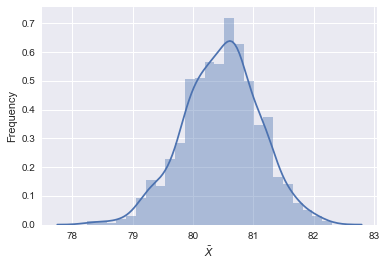
\includegraphics[width=\linewidth]{va13.png} &
    \lstinline[]$assert 80 < boot_mean_mean < 81$\\
    \bottomrule
  \end{tabular}
  \label{tab:va-dist-check}
\end{table}

The visualization in VA13 displays the distribution of bootstrapped sample means as a histogram with a superimposed kernel density estimate (KDE) curve, illustrating the central tendency and variability of the bootstrapped means.

Bootstrapped sample means are calculated by repeatedly resampling the original dataset with replacement and computing the mean for each resampled dataset. This process generates a distribution of the mean, known as the bootstrap distribution, which helps in estimating the variability and central tendency of the original dataset's mean.

The corresponding assertion checks whether the bootstrapped mean lies between 80 and 81, ensuring that the statistical estimation is consistent with expected values. This validation is crucial for confirming the reliability of the bootstrapped estimates and the accuracy of statistical conclusions.

\highlight{\textbf{Finding 3.1} One visualization is used to display the distribution of bootstrapped sample means. The corresponding assertion checks if the bootstrapped mean lies between a specific range, ensuring a consistent statistical estimation.}

\subsubsection{Data Validation ($N = 9$)}

\begin{longtable}{@{} m{0.05\textwidth} m{0.4\textwidth} m{0.4\textwidth} @{}}
  \caption{VA pairs used for data validation.} \\
  \toprule
  \emph{\textbf{Key}} &
  \emph{\textbf{Visual Output}} &
  \emph{\textbf{Assertion}}\\
  \midrule
  \endfirsthead

  \caption[]{VA pairs used for data validation (continued).} \\
  \toprule
  \emph{\textbf{Key}} &
  \emph{\textbf{Visual Output}} &
  \emph{\textbf{Assertion}}\\
  \midrule
  \endhead

  \midrule
  \endfoot

  \bottomrule
  \endlastfoot

  VA30 &
  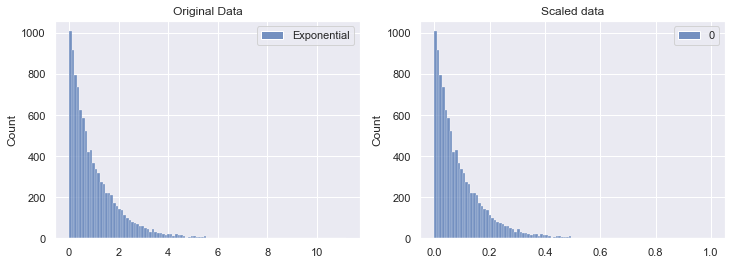
\includegraphics[width=\linewidth]{va30.png} &
  \lstinline[]$assert scaled_data[scaled_data.argmax()] <= 1$\\

  V35 &
  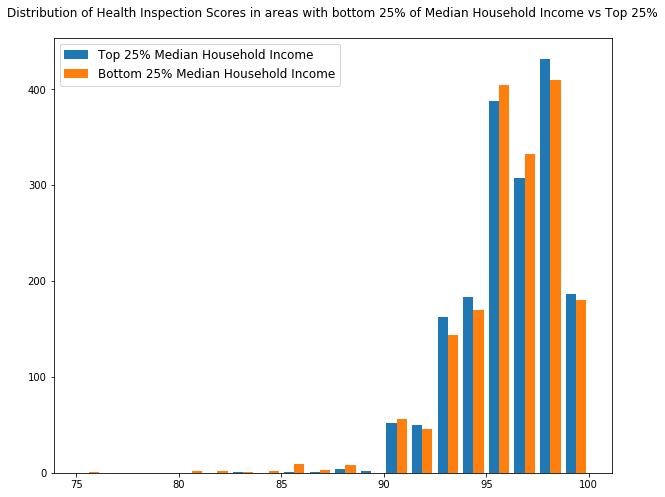
\includegraphics[width=\linewidth]{va35.png} &
  \lstinline[]$assert(all(df_lower['inspection_score'] > 75))$\\

  V57 &
  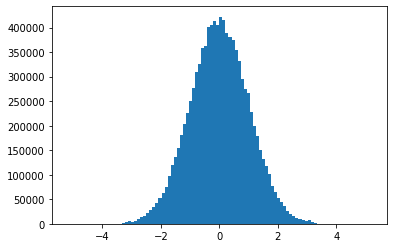
\includegraphics[width=\linewidth]{va57.png} &
  \lstinline[]$assert kstest(data_transformed[:, feature], 'norm').statistic < 1e-2$\\

  VA62 &
  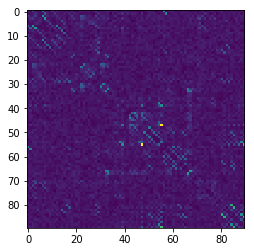
\includegraphics[width=\linewidth]{va62.png} &
  \lstinline[]$assert not np.allclose(x_aug, x_original)$\\

\end{longtable}\label{tab:va-data-validatio}

The VA pairs in Table~\ref{tab:va-data-validatio} collectively illustrate various data validation techniques essential for ensuring the integrity and quality of data used in ML models. 

The visualization in VA30 consists of two histograms comparing the original and scaled distributions of an exponential dataset. The left plot shows the distribution of the original data, while the right plot displays the distribution after scaling. The scaling process adjusts the data to fall within a specified range of 0 and 1. The corresponding assertion checks whether the maximum value in the scaled data is less than or equal to 1, ensuring that the scaling procedure was applied correctly.

The visualization in VA35 shows the distribution of health inspection scores in areas with the bottom 25\% and top 25\% of median household income. The blue bars represent areas with the top 25\% median household income, while the orange bars represent areas with the bottom 25\%. This comparison helps identify any disparities in health inspection scores based on income levels. The corresponding assertion checks that all inspection scores in the lower-income areas are above 75, ensuring that the data reflects a minimum standard of health inspection scores in these areas.

The visualization in VA57 shows a histogram of transformed data after it has been normalised. The corresponding assertion checks that the Kolmogorov-Smirnov (KS) test statistic for the transformed data is less than $1 \times 10^{-2}$, ensuring that the data closely follows a normal distribution.

The visualization in VA62 displays a heatmap of an augmented dataset generated using a weighted k-nearest-neighbors (k-NN) method. This heatmap helps in visualizing the differences and similarities between the original and augmented data. The corresponding assertion checks that the augmented data \lstinline{x_aug} is not nearly identical to the original data \lstinline{x_original}, ensuring that the data augmentation process has introduced sufficient variability.

These validations are crucial for confirming that data preprocessing techniques such as scaling, transformation, and augmentation have been correctly applied. Ensuring the integrity and quality of the data is essential for the subsequent steps in the machine learning pipeline, as it directly impacts the robustness, reliability, and generalization of the models developed. By validating these steps, we can maintain high standards of data quality and model performance, which are fundamental for accurate and meaningful analyses.

\highlight{\textbf{Finding 3.3} Nine VA pairs focus on data validation tasks such as comparing the original with the scaled data distribution and ensuring augmented data is different from the original. These validations confirm that data preprocessing steps like scaling, transformation, and augmentation are correctly applied.}

\section{Discussion}\label{sec:discuss}

Our results from RQ1 reveal that outputs from code cells in Jupyter notebooks are extensively used to make design and implementation decisions during the ML development cycle. Making such decisions however, requires manual validation of the outputs. For instance, we find several instances where practitioners use visualisations to check data distributions and print statements to verify data shapes and types before proceeding with model training. Critical decisions, such as deciding whether to normalize features based on their distributions or adjusting model parameters based on training feedback, rely heavily on these manual checks. Like traditional software systems, an ML pipeline is subject to change due to evolving model requirements, personnel turnover, and changes in the data itself. Such changes can introduce inconsistencies or errors that manual checks might miss, highlighting the need for more automated validation mechanisms. 

Assertions can play a crucial role in automatically validating critical assumptions in ML workflows. As seen in the results from RQ2, assertions can verify that data distributions remain consistent with expectations or that model performance metrics meet predefined thresholds. Embedding assertions into the code helps ensure that any deviation from expected conditions is promptly flagged, reducing the reliance on manual verification and enhancing the robustness and maintainability of ML pipelines. Assertions also serve as an executable form of documentation that captures the assumptions and decisions made during model development. This is particularly important in collaborative environments where multiple practitioners might work on the same project. Assertions ensure that all team members have a clear understanding of the requirements and constraints across the entire ML pipeline, facilitating smoother transitions and handovers. Moreover, they enhance the reproducibility of ML experiments by ensuring that the same validation checks are applied consistently, regardless of the execution order of the notebook cells.

% P71 highlights the lack of proper software engineering best practices within Jupyter notebooks. This shortcoming in computational notebooks has been identified by prior studies~\cite{quaranta2021kgtorrent, pimentel2019large-scale}. In this case study, managing dependencies through external tools is recommended. Python's built-in \emph{requirements.txt}~\footnote{https://pip.pypa.io/en/stable/reference/requirements-file-format/} file allows specifying dependencies and versions. Alternatively, external programs like \emph{pipenv}~\footnote{https://pipenv.pypa.io/en/latest/} and \emph{poetry}~\footnote{https://python-poetry.org/} use lockfiles to ensure specific version control, guaranteeing reproducibility across different systems. 

% NOTE: here we need to bring in prior literature on ML testing; and how majority of the research is working on testing using a test dataset; however we also have data and models
% NOTE: 3 pillars of of ML (sato2019continuous)

From the 3M Jupyter notebooks collected in this study, only 30K (9.7\%) were found to utilize assertions. This indicates that while the use of assertions in Jupyter notebooks is still uncommon, it represents an emerging testing practice within the ML community. The relatively low adoption rate suggests that there is significant room for growth and improvement in the integration of assertions into ML development workflows.

We believe this limited use of assertions is due to a lack of knowledge among practitioners regarding testing approaches and the absence of adequate tooling to support the assertion of data and model properties. Current guidelines on ML coding practices require enhancement to emphasize the importance of testing. There is a pressing need to steer education and research in Software Engineering towards addressing the specific challenges faced when developing ML-enabled software systems. Fostering a deeper understanding of testing practices and providing tools tailored to ML development can help promote more rigorous and reliable testing methodologies within the community.

The assertions presented in RQ2 and RQ3 further reveal two significant challenges in the current landscape of testing in ML Jupyter notebooks. First, the assertions identified in this study lack the support of dedicated testing libraries. This suggests that the culture of testing ML code is still in its infancy, and ML practitioners are not yet fully exploring or leveraging software testing libraries. Secondly, existing testing libraries are not specifically tuned to the needs of ML code, leading practitioners to rely on basic built-in approaches. This highlights the necessity for developing specialized testing frameworks that cater to the unique requirements of ML projects.

Visualizations are an effective tool for interpreting complex ML models and data transformations. However, the manual effort required to validate insights derived from these visualizations can be substantially more compared to text output such as the ones presented in Section~\ref{sec:result-rq2}. We argue that the need for translating visual insights into formal assertions is more pressing. The visual cue and trends observed in visualisations are open to iterpretation, thus the interpretation of the same plot may differ amongst two practitioners. Translating visual insights into assertions ensures taht the knowledge encapsulated in the visualisations along with its interpretation and subsequent decisions made based on this interpretation is preserved and consistently applied throughout the ML lifecycle.

In the VA pairs from RQ3, we see several examples of assertions that fail to capture all the information gained from its visual counter-part. This can lead to a mismatch of expectations in future versions of the ML software. For instance, another project collaborator might run the code with a new version of the dataset or a different learning technique and assume that if the assertions run successfully, the expected patterns from the visualisation are also satisfied. The VA pairs presented in Section~\ref{sec:result-rq3} show that deriving assertions from visualisations is not trivial. Basic visualisation patterns require complex mathematical techniques which may be beyond the expertise of an ML developer. For example, a linear correlation between the true and predicted labels is evident in VA107 presented in Table~\ref{tab:va-model-perf}. Yet, its formal assertion necessitates defining an appropriate threshold for the coefficient of determination metric. Our results show that current software testing practices fail to capture the idiosyncrasies of ML code. There is a pressing need for automated tools, that bridge the disparity between the qualitative evaluation of ML systems using visualisations and the extraction of analytical assertions from these visuals.

% TODO: integrate our NLBSE paper
Our results show a clear need for developing ML-specific testing tools. Such tools should seamlessly integrate with computational notebooks and provide automated suggestions for assertions can greatly enhance the reliability and robustness of ML models. These tools can also aid in documenting and standardizing the use of domain-specific "magic" thresholds, ensuring that they are consistently applied and maintained.

% NOTE: we find overlap between the manual tests performed using the output of code cells and the assertions.

% NOTE: bring in prior work on reproducibility, code quality here
% NOTE: notebooks have been adopted by a much larger scientific community; not eveybody has a background in software engineering; we need more tools to aid notebook users...



\section{Implications}

\paragraph{\textbf{For ML developers}} ML developers are strongly encouraged to incorporate assertions into their Jupyter notebooks. Assertions play a crucial role in validating critical assumptions automatically, reducing the reliance on manual checks, and enhancing the robustness and maintainability of ML pipelines. By embedding assertions, developers can document the decisions made during model development, ensuring that these decisions are consistently applied and preserved throughout the ML lifecycle. This practice not only facilitates smoother transitions and handovers in collaborative environments but also improves the reproducibility of ML experiments by ensuring consistent validation checks.

\paragraph{\textbf{For Researchers}} The use of assertions in Jupyter notebooks, though currently uncommon, is an emerging testing practice within the ML community. This study highlights the potential for assertions to enhance the reliability and robustness of ML models by automating the validation of critical assumptions. Researchers are encouraged to explore the development and evaluation of ML-specific testing methodologies that leverage assertions. This could involve creating new testing frameworks and tools tailored to the unique challenges of ML systems, thus contributing to the advancement of software engineering practices in the ML domain.

\paragraph{\textbf{For Notebook Tool Developers}} There is a clear need for automated tools that suggest assertions based on the outputs of code cells in Jupyter notebooks. Tool developers can play a pivotal role by creating ML-specific testing tools that seamlessly integrate with computational notebooks. These tools should provide automated suggestions for assertions, helping practitioners to translate visual insights into formal, executable checks. By bridging the gap between qualitative evaluation and analytical assertions, such tools can significantly enhance the reliability and robustness of ML models, ensuring that they meet predefined performance standards consistently.

\paragraph{\textbf{For Educators}} Educators should emphasize the importance of testing ML code written in Jupyter notebooks as part of the curriculum. By incorporating testing practices and the use of assertions into ML education, students can develop a deeper understanding of the importance of automated validation in ensuring model reliability and robustness. Teaching these best practices early on can help cultivate a culture of rigorous testing among future ML practitioners, preparing them to address the specific challenges faced in ML-enabled software systems.

\paragraph{\textbf{For General Notebook Users}} Awareness of software engineering best practices, including the use of assertions, is crucial for all users of Jupyter notebooks. Assertions serve as an executable form of documentation, capturing the critical assumptions and decisions made during the development process. By adopting assertions, users can ensure that their notebooks are more robust, maintainable, and reproducible. This practice helps in maintaining consistency and reliability, especially in collaborative projects where multiple users might work on the same notebook, ensuring that the assumptions and validations are transparent and consistently applied.

\section{Future Work}

\section{Conclusion}

% BibTeX users please use one of
% \bibliographystyle{spbasic}      % basic style, author-year citations
\bibliographystyle{spmpsci}      % mathematics and physical sciences
%\bibliographystyle{spphys}       % APS-like style for physics
\bibliography{bibliography}   % name your BibTeX data base

\end{document}
% end of file template.tex

